\renewcommand*\thesubsubsection{\arabic{section}.\arabic{subsection}.\arabic{subsubsection}}
\setlength{\abovecaptionskip}{0pt plus 0pt minus 0pt} % Chosen fairly arbitrarily

\chapter{Experiments and results}\label{ch:5}

In this chapter, we will go through all notable\footnote{We only present a subset of conducted experiments that are implemented in the msc-neuro repository. Further, the experiments are reordered and their naming scheme does not directly correspond between the repository and the text of this thesis. For matching, refer to msc-neuro/experiments/readme.md. Similarly, we only provide a subset of figures that were created for analysis.} experiments and their results. It is divided into three sections. First, we focus on reimplementing, assessing, and improving the HSM model by \cite{antolik} Second, we compare its DoG layer contribution with various less constrained variants from classical deep learning and also assess the separable layer introduced by \cite{klindt}. Lastly, we explore pooling the three regions of our dataset together for a single shared model as well as test the best architectures on each of the regions separately.


\section{Assessment and improvements of HSM}

In this section, we start by listing the differences between the original HSM model by \citeauthor{antolik} and our reimplementation. Then, we move towards experiments focused on the effects of training regime hyperparameters on both best achieved performance and also model stability. We finish with an initial look at soft regularizations and additional non-linearity.

\addtocounter{subsection}{-1} % Make differences 0 so that experiments start from 1.1.1 %
\subsection{Differences introduced by reimplementation}\label{ch:5.1.0}

We started by reimplementing the HSM model by Antolik et al. Due to the differences between the tools available in the general-purpose deep learning framework Theano, that was originally used by the model’s authors, and the neuroscience-focused toolkit NDN3, used by us, we could not create an exact replica. Nor was exact recreation desirable due to the availability of more recent components such as modern optimizers\footnote{\cite{2016arXiv160904747R}}.

Most notably, the originally used fitting method, the Newton Conjugate-Gradient algorithm (see section \ref{ch:2.1.3}), is not available in NDN3. Instead, we opted for ADAM (\cite{kingma2014adam}), a stochastic gradient descent based method introduced in 2014, and generally considered as the current go-to\footnote{Even though its dominance is being questioned \cite{2019arXiv191005446C}.} optimizer for DNN models. This change forced us to deviate in the training regime as well. While the original model worked on full training set batches, ADAM is commonly used with appropriately sized mini-batches\footnote{\cite{2017arXiv170508741H}, \cite{2017arXiv171100489S}.}. After a few initial tests, we empirically decided on 16 as our initial batch size - balancing expected model performance and computational efficiency. The same way, we chose to start with a learning rate of 0.0001. The last impact of a different optimization method was that unlike with Newton Conjugate-Gradient, all of our weight bounds, including those for Difference of Gaussians (DoG) layer, were enforced only on random initialization while the original optimizer restricted their values to stay within those bounds throughout the training as well.

The second difference between our reimplementation and the original model was in initialization of weights and biases. While we copied the way DoG layer weights are initialized - both in terms of bounds and distributions, for both fully connected layers - hidden and output - as well as the bias of DoG layer, we opted for the initialization schema already provided by NDN3. Instead of the original uniform distribution with relatively wide bounds, normal distribution scaled to 0.1 variance and 0 mean was used for weights, and plain zeroes were used for biases\footnote{\cite{glorot}}. The last difference was in input. In an initial exploration phase, we discovered that the original range of stimuli data (0-0.000255) led to very poor training performance. Thus, we opted for rescaling it to what we assume was the intended range: 0-255.

\subsection{Reimplementation}
\subsubsection{Initial reimplementation: Baseline 1}

With aforementioned differences, the initial reimplementation, further referred to as \emph{baseline 1}\footnote{For explanation what baseline refers to, see section \ref{ch:4.2.1}.} model, achieved validation set correlation of 0.42, 0.48, and 0.3 for its median, 90th percentile, and 10th percentile runs by the end of the 35 000 epochs of training respectively. As shown on figure \ref{fig:5.1.1.1}, this is worse than the fully trained results reported by \citeauthor{antolik} (0.48, 0.5, 0.44) in both top percentile performance but also the variance with respect to random initializations, demonstrating the sensitivity of DNN models to even minor changes.

\begin{figure}[H]
    \centering
    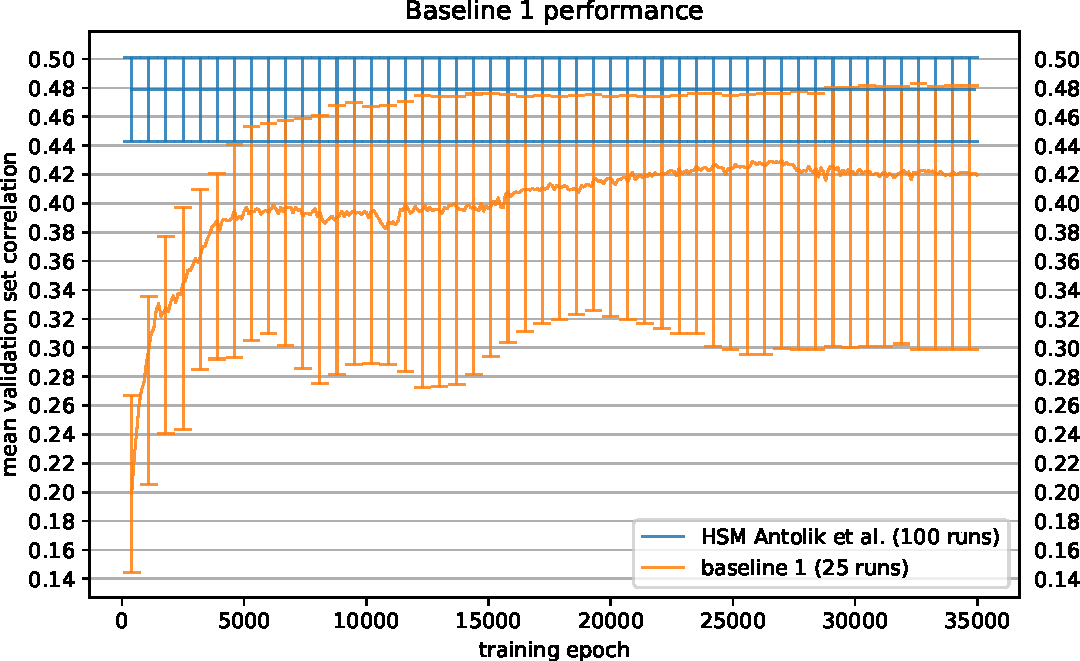
\includegraphics[width=1\textwidth]{../figures/05_1_1_1}
    \caption[Experiment 1.1.1]{Validation set correlation of first baseline model versus the original \cite{antolik} implementation on region 1\protect\footnotemark.}
    \label{fig:5.1.1.1}
\end{figure}
\footnotetext{We only have fully trained data for the original implementation. We thus show the final mean performance and its variance for all time points.}

\subsection{Training hyperparameters tuning}
\subsubsection{Input scaling: Baseline 2}
Informed by the recommended\footnote{\cite{10.5555/645754.668382}} practise of data normalisation, \emph{experiment 1.2.1} focused on input scaling\footnote{Input scaling can have big influence despite the fact that both the first DoG layer and the two subsequent fully connected layers of the model should be able to learn arbitrary linear transformation through the combination of multiplicative weights and additive biases.}. Two different variations were tested. First, where only the input is linearly normalized to have 0 mean and standard deviation of 1. And second, where input is scaled the same way but the output is also scaled to have standard deviation of 1. We could not shift the mean of the output to 0 because that would cause some outputs to be negative and go against our Poisson noise assumption\footnote{Refer to section \ref{ch:1.4.1}.}.

\begin{figure}[H]
    \centering
    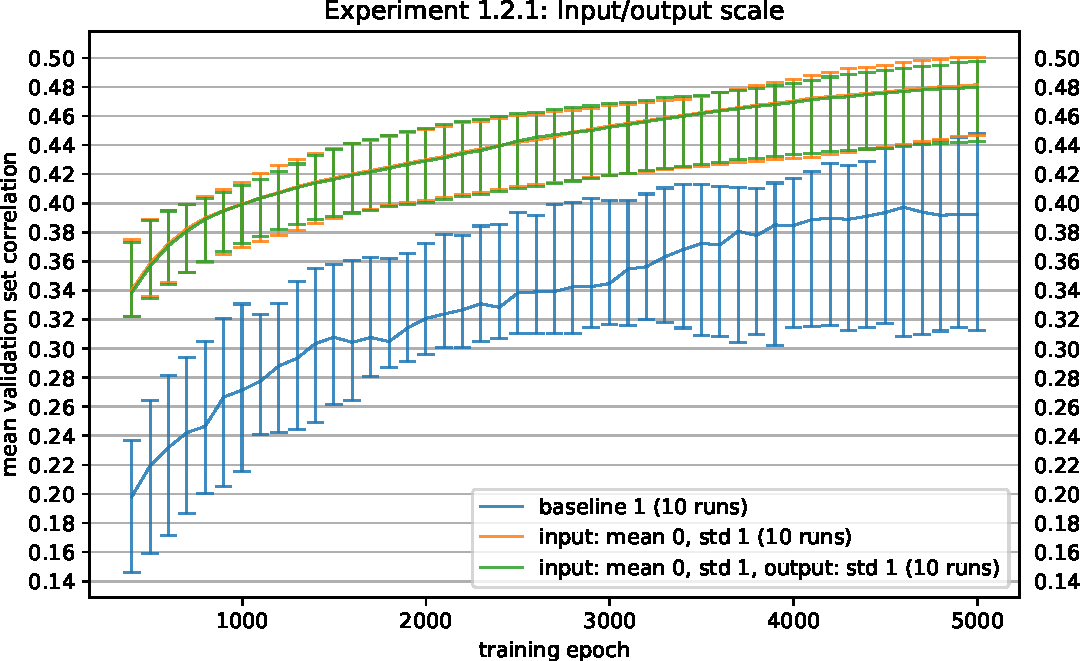
\includegraphics[width=1\textwidth]{../figures/05_1_2_1}
    \caption[Experiment 1.2.1]{Results of baseline 1 versus normalised inputs\protect\footnotemark.}
    \label{fig:5.1.2.1}
\end{figure}
\footnotetext{Unlike the previous figure, this is restricted to 5 000 epochs and 10 runs per experiment instance (refer to section \ref{ch:4.4}).}

Figure \ref{fig:5.1.2.1} showcases the dramatic improvement both of these changes had in both 90th percentile run performance but especially stability. Both achieved validation set correlation of approximately 0.48, 0.5, and 0.45 for its median, 90th percentile, and 10th percentile runs respectively after only 5000 epochs\footnote{For experiments we are only training for 5000 epochs (refer to section  \ref{ch:4.4}) and so the performance of the \emph{baseline 1} model is not entirely converged yet.} of training, thus improving over the original HSM implementation by Antolik. Out of the two, we have decided to select the simpler one, scaling only input, as our new base model, \emph{baseline 2}. Fully trained comparison on 35 000 epochs between \emph{baseline 1} and the new \emph{baseline 2}, achieving 0.51, 0.52, and 0.49 respectively, is presented by figure \ref{fig:5.1.2.1_2}.

\begin{figure}[H]
    \centering
    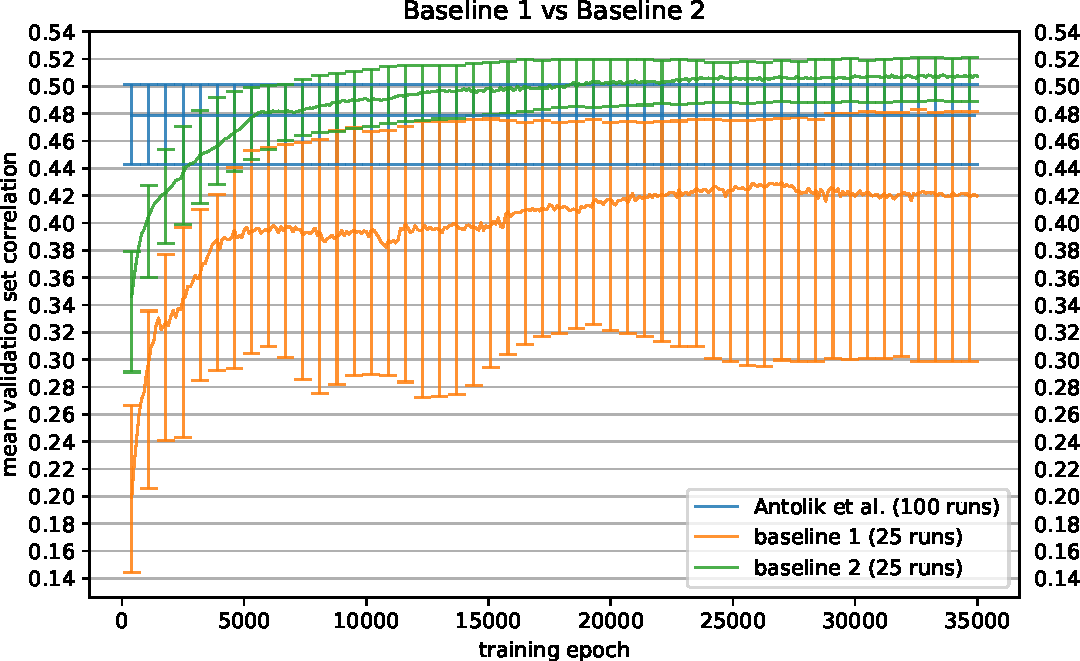
\includegraphics[width=1\textwidth]{../figures/05_1_2_1_2}
    \caption[Experiment 1.2.1 2]{Baseline 1, baseline 2, and \citeauthor{antolik} implementation. Showcasing the effect of small non-architectural changes.}
    \label{fig:5.1.2.1_2}
\end{figure}

\subsubsection{Gaussian versus Poisson}\label{ex:1.2.2}
The \emph{experiment 1.2.2}, based on the \emph{baseline 2} model, tested the impact of our assumptions from the \nameref{ch:1.4.1} section in terms of model performance. In line with our expectations and prior research, the version with Gaussian noise assumption loss function had slightly but consistently worse results of (0.46, 0.47, 0.42) after 5 000 epochs of training (Fig. \ref{fig:5.1.2.2}). 

\subsubsection{Bias initialization}\label{ex:1.2.3}

In \emph{experiment 1.2.3}, we revisited the bias initialization scheme. Instead of the zero initialization chosen for the initial reimplementation\footnote{Refer to section \ref{ch:5.1.0}.} we tested truncated normal initialization\footnote{Refer to section \ref{ch:3.1.1}.} an absolute value of normally distributed samples with 0 mean and 0.1 variance. This was inspired by the presence of strictly positive initialization of biases in the original model. This change proved beneficial (Fig. \ref{fig:5.1.2.2}), yielding a model with generally faster convergence, better median and 10th percentile runs, and only a slightly worse 90th percentile run of (0.48, 0.49, 0.46) after 5 000 epochs of training.

\begin{figure}[H]
    \centering
    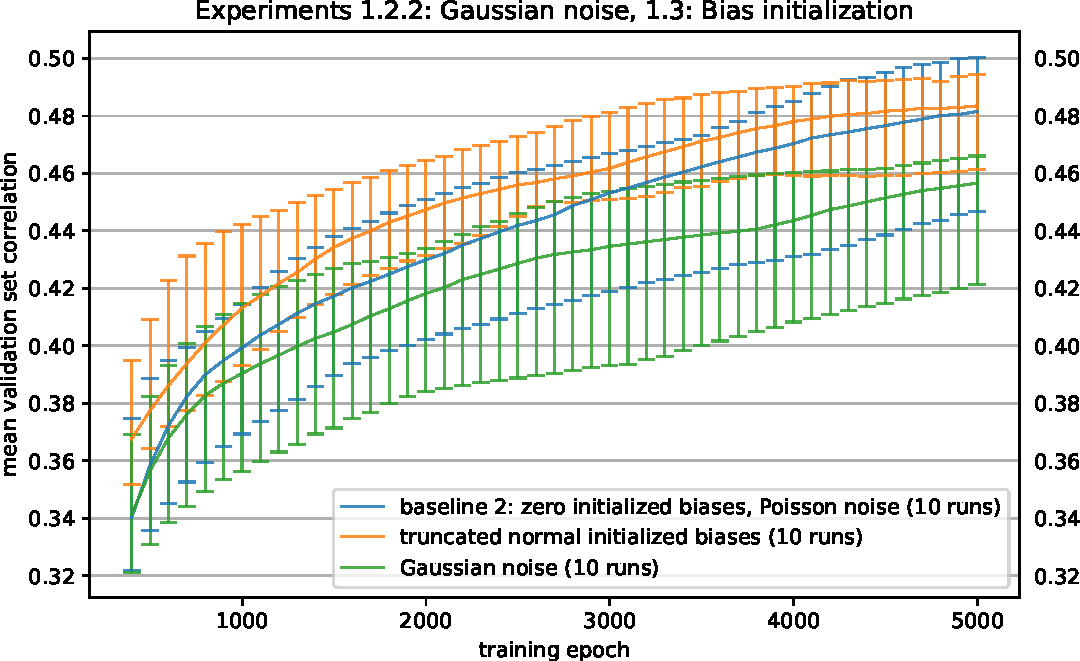
\includegraphics[width=1\textwidth]{../figures/05_1_2_2}
    \caption[Experiments 1.2.2 and 1.2.3]{Impact of gaussian noise and truncated normal initialization of biases (experiments \ref{ex:1.2.2} and \ref{ex:1.2.3}).}
    \label{fig:5.1.2.2}
\end{figure}

\subsubsection{Learning rate}\label{ex:1.2.4}

The \emph{experiment 1.2.4} built upon the foundations of our initial experimentation phase\footnote{Refer to section \ref{ch:5.1.0}.} and systematically tested various learning rates for our ADAM optimiser\footnote{While one might assume ADAM should be relatively stable with respect to various learning rates due to its adaptivity based on first and second moments of the gradient, there is little evidence to support this.}. The best performance was achieved by an order of magnitude higher learning rate - 0.001. It reached correlation of (0.5, 0.51, 0.49) by the end of 5 000 epochs of training (Fig. \ref{fig:5.1.2.4}), substantially increasing overall performance, stability, and also convergence speed over both the previous baseline models and the original HSM implementation by \citeauthor{antolik} Further research could be done into dynamic learning rate schedules such as exponential decay rate or step decay. Similarly, both beta and epsilon hyperparameters of ADAM could be explored\footnote{They were kept on their NDN3 defaults for our experiments.} (\cite{2019arXiv191005446C}).


\begin{figure}[H]
    \centering
    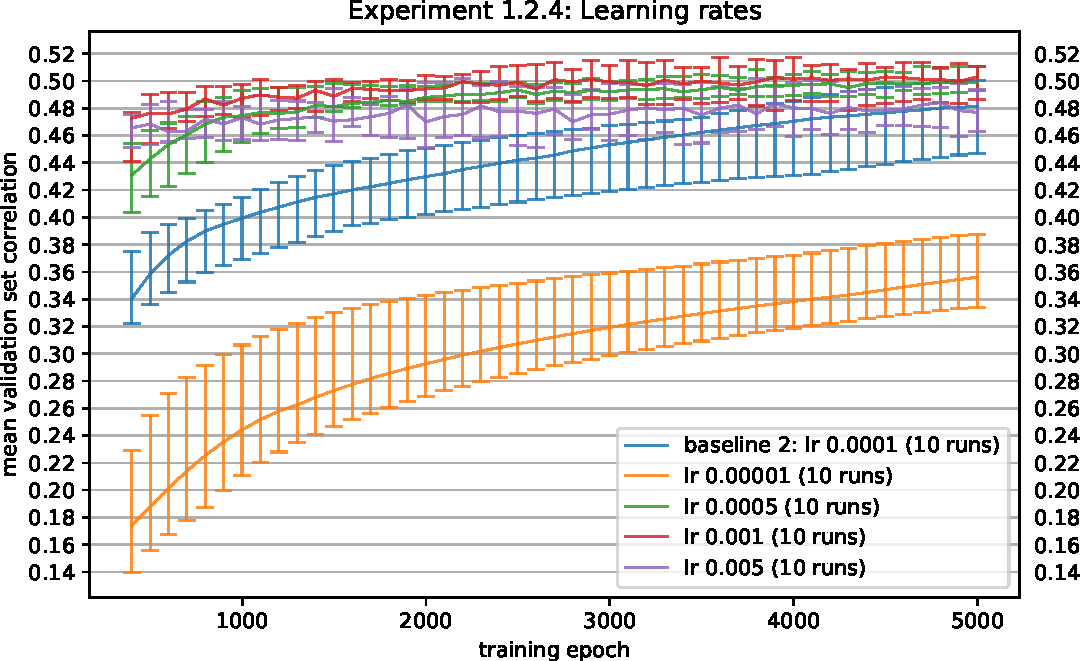
\includegraphics[width=1\textwidth]{../figures/05_1_2_4}
    \caption[Experiment 1.2.4]{Impact of different learning rates.}
    \label{fig:5.1.2.4}
\end{figure}

\subsubsection{Learning rate and bias initialization: Baseline 3}\label{ex:1.2.5}

Combining improvements uncovered by \emph{experiments 1.2.3} and \emph{1.2.4}, we created a new base model, \emph{baseline 3}. Upon training it fully for all 35 000 epochs, we found that the new baseline converged significantly faster and initially with a substantially smaller spread (figure \ref{fig:5.1.2.5}). 

\begin{figure}[H]
    \centering
    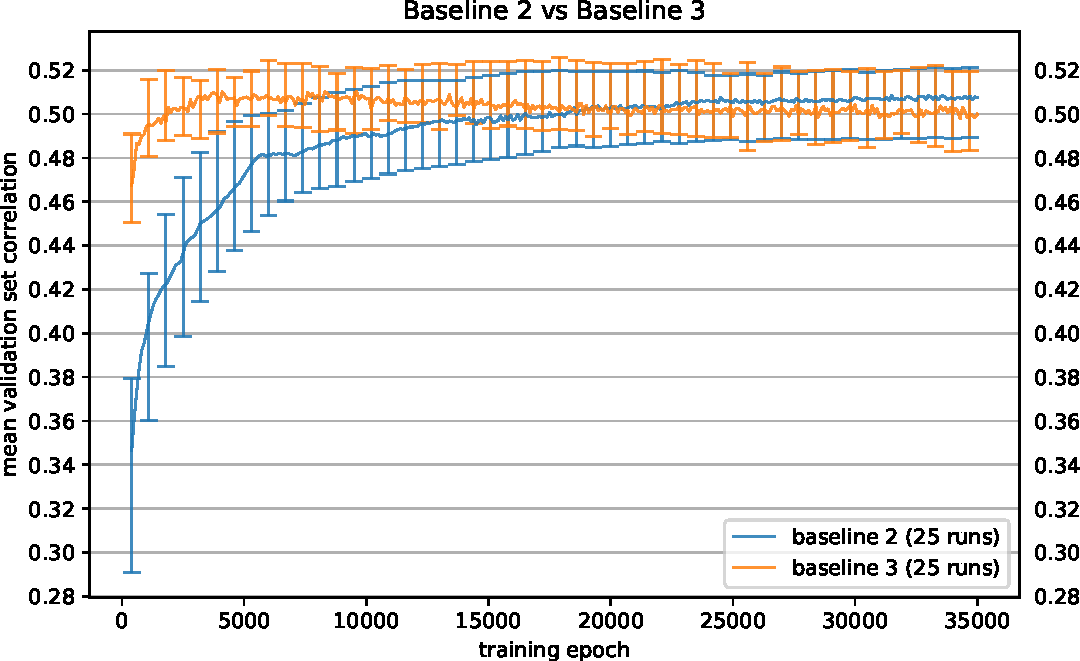
\includegraphics[width=1\textwidth]{../figures/05_1_2_5}
    \caption[Experiment 1.2.5]{Faster convergence, initially smaller spread, and onset of overfitting.}
    \label{fig:5.1.2.5}
\end{figure}

By epoch 6 000 it reached a correlation of (0.507, 0.524, 0.499) versus (0.481, 0.5, 0.454) of \emph{baseline 2} model. Beyond that, however, it started to overfit, eventually falling to (0.5, 0.521, 0.492) versus (0.508, 0.521, 0.49) of \emph{baseline 2} at the end of 35 000 epochs of training. 

Since the peak results were comparable and \emph{baseline 3} showed substantially faster convergence, especially in the 5 000 epochs range - which is important for experiments evaluation, we chose to use it for all further experiments, replacing \emph{baseline 2}.

\subsubsection{Batch size}

Similarly to \textit{1.2.4}, \textit{experiment 1.2.6} systematically reevaluated another training hyperparameter - the batch size. To ensure for fair comparison, throughout the experiment we conserved the number of model updates as opposed to the number of epochs\footnote{For more information about the relationship between the number of updates and batch size, please refer to the section \ref{ch:1.3.2}.}. I.e. with larger batch size and thus less updates per epoch, we scaled the number of epochs up proportionally. For smaller batch sizes, we did not decrease the number of epochs to ensure each data point is evaluated at least a certain number of times.

\begin{figure}[H]
    \centering
    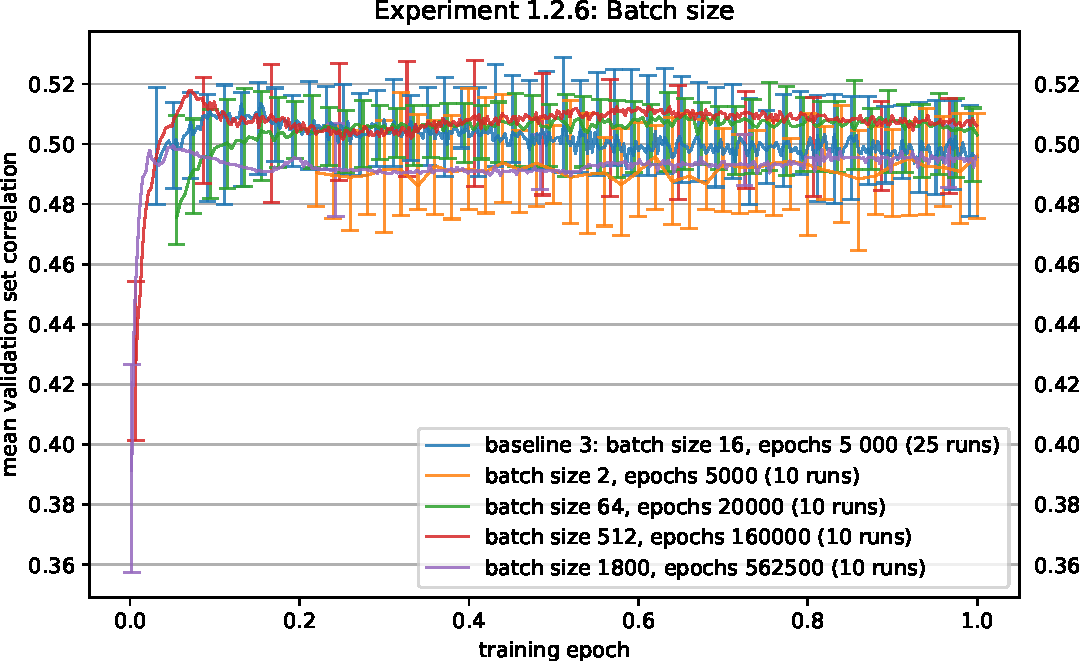
\includegraphics[width=1\textwidth]{../figures/05_1_2_6}
    \caption[Experiment 1.2.6]{Various batch sizes. Training epochs are normalized across instances. 0 being the 0th epoch, 1 corresponding to the last training epoch for that particular instance.}
    \label{fig:5.1.2.6}
\end{figure}

Figure \ref{fig:5.1.2.6} illustrates that batch size had limited impact, with median run performance of all variants between 0.49-0.51 and comparable stability. Both ends of the spectrum, really small batch sizes (2, 4) and the biggest possible (spanning the entire dataset) performed slightly worse than the \textit{baseline 3}. Otherwise, even relatively large batch sizes (512) reached good peak performance\footnote{Even though not unheard of (\cite{2017arXiv171100489S}), it is still a relatively surprising result (\cite{2017arXiv170508741H}).} and actually proved to be slightly more resilient to overfitting. Due to their computational requirements, however, we chose not to change our training regime for further experiments. The variance in performance between intermediately sized batch (16-128 examples) was not significant enough to draw clear conclusions from.

\subsection{Regularizations and non-linearity}
\subsubsection{Dropout}

\textit{Experiment 1.3.1} explored dropout\footnote{Refer to section \ref{ch:1.3.2}.} regularization on the hidden fully connected layer. Since dropout can decrease the effective capacity of the model, we tested three sizes of the hidden layer, the original - 20 \% of the number of output neurons, 30 \% and 40 \%. 

As Figure \ref{fig:5.1.3.1} illustrates, the best result was achieved by the baseline model without any dropout and with the original hidden layer size. The bigger the dropout, the worse performance. Similarly, for weak or moderate dropout, a larger hidden layer led to lower results. Only for strong dropout (50 \%), a bigger hidden layer outperformed smaller one.

\begin{figure}[H]
    \centering
    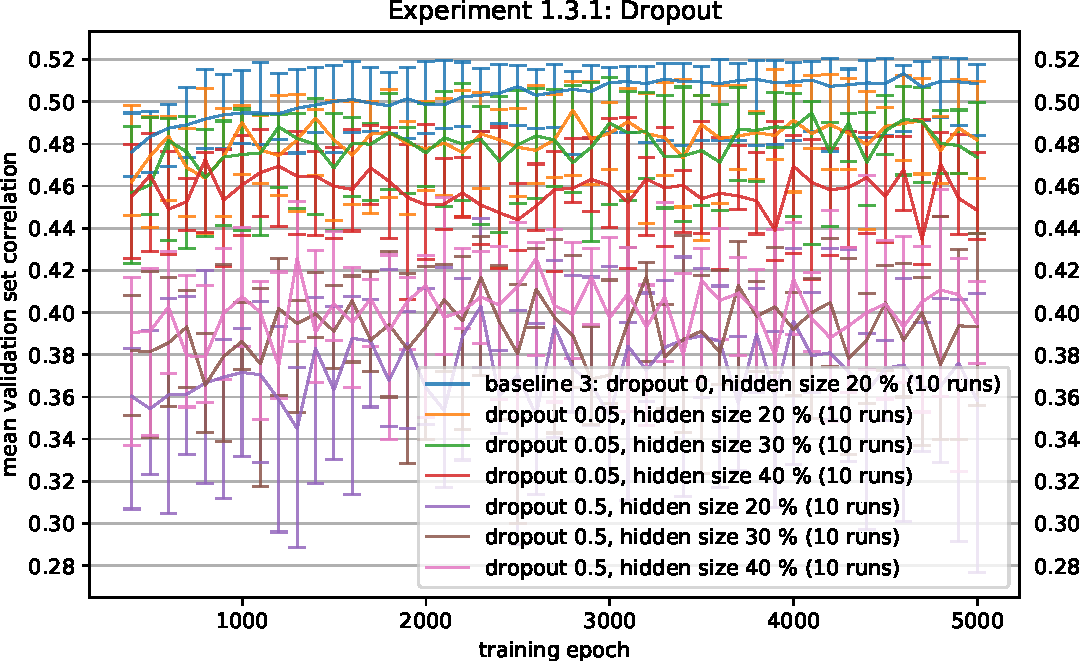
\includegraphics[width=1\textwidth]{../figures/05_1_3_1}
    \caption[Experiment 1.3.1]{Performance loss incurred by dropout regularization (dropout probability) on the hidden layer.}
    \label{fig:5.1.3.1}
\end{figure}

Our working hypothesis for these results is that even light dropout on the hidden layer substantially changes the structure of the network every batch due to the network’s relatively small size. Doing so, it causes significant instability of the gradient and thus disturbs training. This is supported by the observation that the difference in performance cannot be explained just by the smaller capacity of a layer with dropout as this should be more than mitigated by the tested larger variants. The weakest dropout setting drops just one out of the cca. 20 neurons of the hidden layer while the larger variants add cca. 10 and cca. 20 additional neurons respectively. A more thorough exploration would be needed to properly determine the cause, however.

\subsubsection{L1 and L2 regularizations}

\textit{Experiment 1.3.2} tested L1 and L2 regularizations on both fully connected layers together, the hidden as well as the output, in combination with bigger variants of the hidden layer. The results (Fig. \ref{fig:5.1.3.2}) showed too strong regularization, especially L1 type, effectively prevents training. Moderate L2 mitigated the performance loss induced by a larger hidden layer and seemed to improve convergence speed even for the baseline sized hidden layer variant. L1 led to consistently worse results than L2 for this architecture.

\begin{figure}[H]
    \centering
    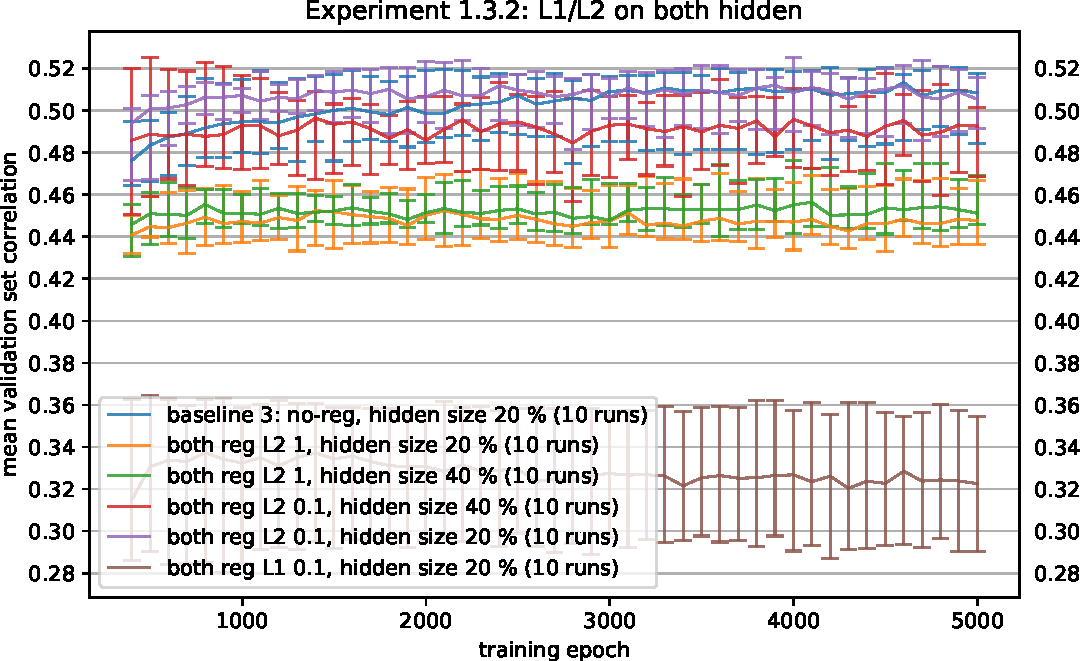
\includegraphics[width=1\textwidth]{../figures/05_1_3_2}
    \caption[Experiment 1.3.2]{Influence of L1 / L2 regularization on both fully connected layers.}
    \label{fig:5.1.3.2}
\end{figure}

\subsubsection{Separate L2 regularizations: Baseline 4}\label{ex:1.3.3}

Informed by \textit{1.3.2}, \textit{experiment 1.3.3}, assessed different strengths of L2 regularization on the hidden and the last layer separately. To fully see the impact on both convergence speed but also overfitting - to which \textit{baseline 3} model was susceptible to\footnote{Refer to experiment \ref{ex:1.2.5}}, we trained this experiment for full 35 000 epochs.

Figure \ref{fig:5.1.3.3} illustrates that moderate L2 regularization on the output layer leads to better results, especially with longer training during which it mitigates overfitting observed on previous models. The best variant reached an end of training, which was also its peak, performance of (0.513, 0.533, 0.506), improving upon \textit{baseline 3} with (0.496, 0.511, 0.489) end of training and (0.508, 0.519, 0.494) peak\footnote{These numbers do not directly match those reported in \ref{ex:1.2.4} because they are computed using only the first 10 runs to enable direct comparison with other experiment instances. Meanwhile, \ref{ex:1.2.4} reports numbers from 25 runs as it is a baselines comparison.} validation set correlation. We used this instance as the new \textit{baseline 4} model (performance comparison on figure \ref{fig:5.1.5}). Furthermore, any L2 regularization on the hidden layer led to worse performance, regardless of the hidden layer size. At best the benefit of last layer regularization canceled out the drawback of hidden layer regularization, leading to \textit{baseline 3} level of performance.

\begin{figure}[H]
    \centering
    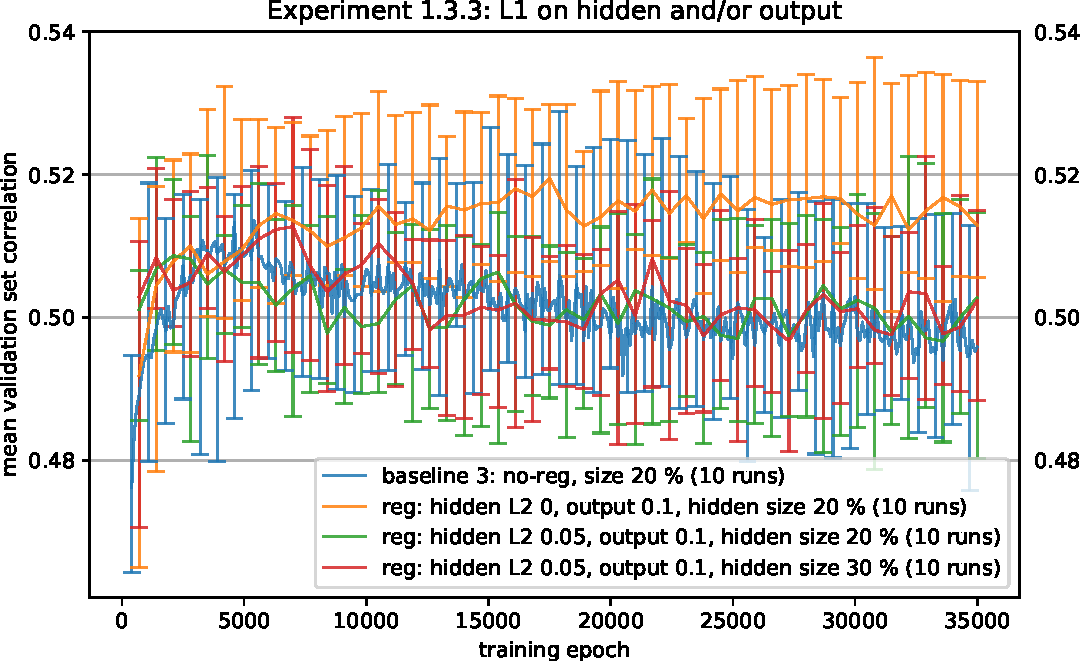
\includegraphics[width=1\textwidth]{../figures/05_1_3_3}
    \caption[Experiment 1.3.3]{Impact of L2 regularization on the output layer with full training.}
    \label{fig:5.1.3.3}
\end{figure}

\subsubsection{DoG layer non-linearity}\label{ex:1.3.4}

\textit{Experiment 1.3.4} explored adding a nonlinearity after the DoG layer. While the linear activation function of the DoG layer in the original HSM model by \cite{antolik} was biologically motivated, more recent studies of V1 modeling frequently feature a cascade of convolutional filters, each followed by a non-linearity. For example, \cite{klindt} - the current state of the art on our dataset, contains 3 convolutional layers and thus 3 non-linearities. Similar architecture can also be seen in \cite{ecker} or \cite{Walke506956}\footnote{More information in section \ref{ch:2.3}.}. The findings of Antolik et al. proved to be correct, however, with the version containing a SoftPlus nonlinearity after the DoG layer achieving a worse result of (0.494, 0.512, 0.467) versus (0.51, 0.527, 0.502) of baseline 4 after 5 000 epochs of training.

\subsection{Input scaling}
\subsubsection{Implicit and explicit input scaling}

Intrigued by the results of \textit{1.2.1}, \textit{experiment 1.4.1} systematically tested the impact of input data scaling and the capability of the model to train its own input transformation. We tested 3 ways of preprocessing the data in combination with an automatic, yet explicit, trainable scaling added to the model. The three modes of preprocessing were: the original scale (0-0.000255), our initial scale (0-255), and the - since \textit{baseline 2} used - normalisation to 0 mean and 1 standard deviation. Each variant was assessed with and without an additional linear scale layer\footnote{Refer to section \ref{ch:3.1.1}.} prepended as the first layer of the model. The experiment was conducted with a baseline 3 model\footnote{This is a consequence of not presenting the results in the order the experiments were conducted. We, however, believe it does not diminish the interpretation of the results in any way.}.

The idea behind the linear scale layer was that if there was an explicit layer with just two parameters that is only capable of linear transformation of the whole input at once, it should be able to learn any scale relatively easily. Thus achieving close to or exceeding the baseline performance, regardless of the input data preprocessing. And if not that, it at least should not lead to worse results as it should be able to stay at its initial parameters, which were initialized to 1 for the multiplicative weight and 0 for the additive bias.

\begin{figure}[H]
    \centering
    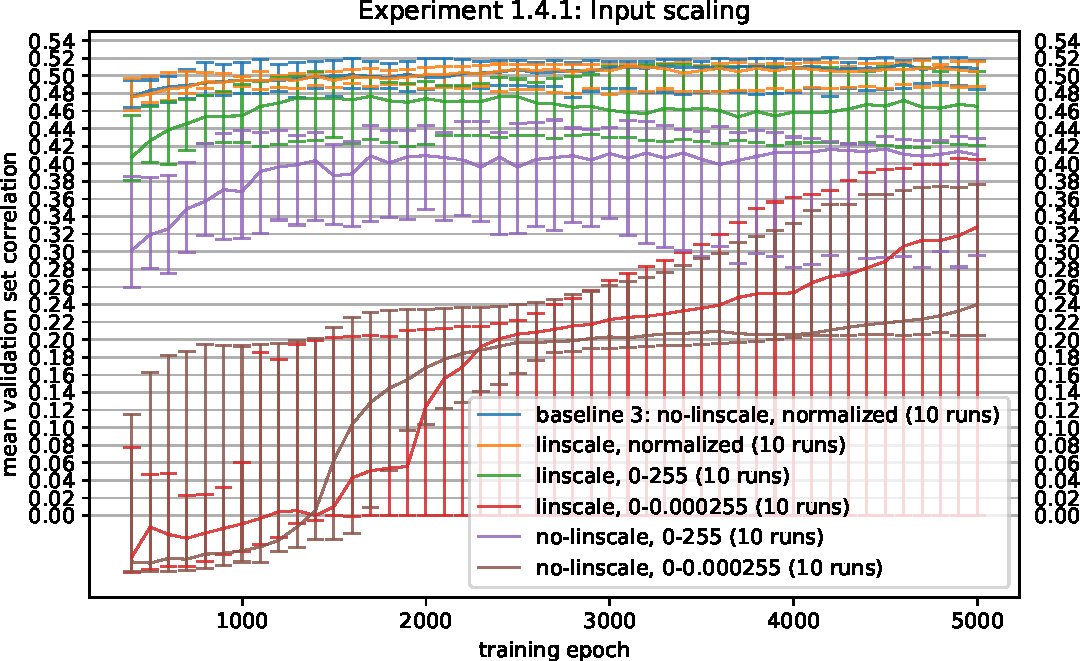
\includegraphics[width=1\textwidth]{../figures/05_1_4_1}
    \caption[Experiment 1.4.1]{Impact of input scaling and explicit linear scale layer.}
    \label{fig:5.1.4.1}
\end{figure}

As illustrated by figure \ref{fig:5.1.4.1}, adding an explicit linear scale layer improved the results of both not-normalized versions of input preprocessing. The integer variant (range 0-255) achieved levels of performance higher (0.465, 0.505, 0.421) than its non-linear layer scale variant (0.41, 0.429, 0.295) but lower than the normalised baseline (0.509, 0.517, 0.484). Thus not proving our hypothesis that the linear scale layer might effectively learn any transformation - even the normalisation. Similarly, for the not pre-processed variant (0-0.000255), the explicit scale layer enabled large gains in both 50th and 90th percentile runs but did not improve on the baseline\footnote{We are aware that the original scale version with an explicit input scale layer does not show its full potential within the 5 000 epochs of training. There is, however, no reason to believe its peak performance would be substantially higher.}. Notably, its 10th percentile was worse, hinting at the possibility that for extreme distributions of the input data additional free parameters with large effect can lead to unrecoverable training when paired with certain initializations.

For already normalized input, both variations with and without the prepended linear scale layer fared indistinguishably. That does not mean normalizing is the best possible scale for our data. As shown by this very experiment, our linear scale layer cannot always find global optima, and so the absence of a better result with it versus without it does not prove anything, globally. But it at least suggests normalizing might be a decent local optimum for our model, an observation in line with literature (\cite{Goodfellow-et-al-2016}, \cite{Jin2015}).


\subsection{Discussion}
That concludes the initial set of experiments focused on training hyperparameters, fully connected layers regularization, and generally smaller changes to the original HSM architecture by \citeauthor{antolik}. It showed a few things. First, non-architectural hyperparameters such as learning rate or input data scale can have substantial impact and should always be thoroughly tested. Similarly, a single additional non-linearity can have negative influence despite it being part of related state of the art architectures. 

We also observed that both the median performance and the stability of a model with respect to parameters initializations can differ widely, even for the same or very similar architecture. Through non-architectural changes only\footnote{Adding an L2 regularization on the hidden layer influences only parameters fitting, and so we do not consider it an architectural change in this context.}, we managed to decrease the difference between 90th and 10th percentile runs from 0.18, with \textit{baseline 1} model, to 0.03 of \textit{baseline 4}, while also increasing the median run performance by 0.05 (Fig. \ref{fig:5.1.5}, table \ref{tab:5.1.5}). As a byproduct, this also revealed that analysing a single run with a particular random initialization might paint an incorrect picture. A problem best shown by the 10th percentile run of an \textit{experiment 1.4.1} instance - that did not train at all while its 50th percentile run fared decently, but by far not limited to only our model or dataset (\cite{2019arXiv190910447M}).

\setlength{\abovecaptionskip}{10pt plus 0pt minus 0pt} % Chosen fairly arbitrarily
\begin{table}[H]
    \renewcommand{\arraystretch}{1.0}
    \centering
    \begin{tabular}{l|l|l|l|l|l|l}
        \toprule
        \textbf{Percentile:} & \textbf{50th} & \textbf{90th} & \textbf{10th} & \textbf{50th} & \textbf{90th} & \textbf{10th} \\
        \textbf{Epochs:} & \textbf{5k} & \textbf{5k} & \textbf{5k} & \textbf{35k} & \textbf{35k}& \textbf{35k} \\ \midrule
        Baseline 1 & 0.395 & 0.449 & 0.299 & 0.42 & 0.48 & 0.3 \\ 
        HSM \citeauthor{antolik} & - & - & - & 0.48 & 0.50 & 0.44 \\ 
        Baseline 2 & 0.472 & 0.499 & 0.444 & 0.508 & 0.521 & 0.49 \\ 
        Baseline 3 & 0.507 & 0.517 & 0.498 & 0.5 & 0.521 & 0.492 \\ 
        Baseline 4 & 0.511 & 0.527 & 0.495 & 0.514 & 0.531 & 0.498 \\ \bottomrule
    \end{tabular}
    \caption[Evaluation of 5k/35k epochs training on region 1]{Evaluation set correlation on region 1 across baseline models using 25 runs. Performance at epoch 5 000 and 35 000 is shown\protect\footnotemark. }
    \label{tab:5.1.5}
    \renewcommand{\arraystretch}{1.0}
\end{table}
\footnotetext{For the \citeauthor{antolik} model we only have the end of training data.}
\setlength{\abovecaptionskip}{0pt plus 0pt minus 0pt} % Chosen fairly arbitrarily

\begin{figure}[H]
    \centering
    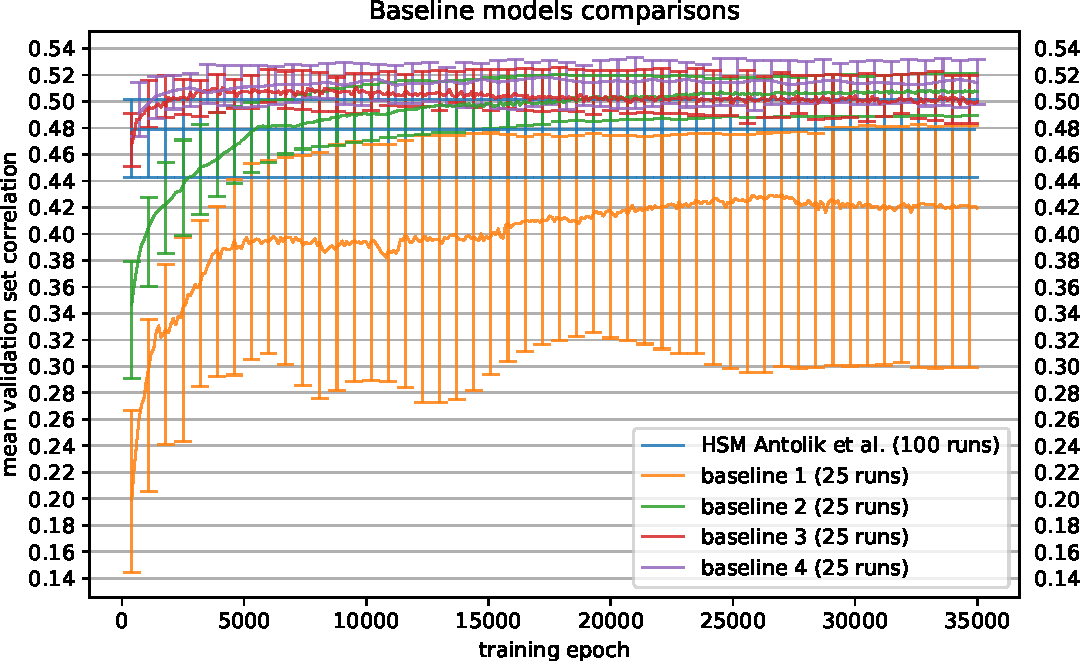
\includegraphics[width=1\textwidth]{../figures/05_1_5_1}
    \caption[Baseline models on region 1]{Evaluation set correlation on region 1 across baseline models.}
    \label{fig:5.1.5}
\end{figure}

Lastly, we significantly improved convergence speed. While the original model by Antolik et al. did 1 800 000 000 datapoint evaluations\footnote{100 epochs, each with 10 000 evaluations, using the whole dataset (1800 in case of region 1) batch.}, our model managed with 1/200th of that: 9 000 000, assuming training for 5 000 epochs - the setting we use to evaluate experiments. If we limited ourselves further, to only 1 000 epochs - still getting a decent performance of (0.514, 0.531, 0.498) on baseline 4 model, it would only need 1/1000th of data-point evaluations. While less impressive, our model is better even in terms of the number of model updates - with requiring roughly half of the original (1 000 000 vs 565 000\footnote{Assuming 5 000 epochs and batch size 16.}) implementation.

\section{Variations on the filter and hidden layers}
In this section, we examine larger architectural changes of the HSM model, focusing on its first two layers - filter and hidden. We compare biologically inspired techniques that feature hard regularizations to more generic methods from classical deep learning with soft regularizations. We start with fully connected layers, drawing parallels to classical LNLN and LN models, and then move to convolution layer, convolutional variants of the DoG layer, and also the separable layer introduced by \cite{klindt} Unless explicitly specified, all experiments in this section were conducted with a \textit{baseline 4} model.

\subsection{Fully connected models}
\subsubsection{LNLN model}\label{ex:2.1.1}

\textit{Experiment 2.1.1} explored replacing the first two layers, the DoG filter and the fully connected hidden, with a single fully connected layer. This created an architecture equivalent to an LNLN model\footnote{For more information refer to section \ref{ch:1.2.2}.}. Two fully connected layers, the first serving as a set of filters and the second predicting neural response through per output neuron combination of said filters’ outputs. The same as in an LNLN model, both fully connected layers were followed by a SoftPlus nonlinearity. Inspired by the hard regularization properties of the DoG layer\footnote{The resulting difference-of-Gaussians filters are by construction spatially smooth.}, the filter layer featured a Laplacian regularization to ensure spatial smoothness of the filters and the output layer an L2 regularization, as it showed to be beneficial in experiment \ref{ex:1.3.3}.

This experiment was not just to test a completely different architecture. Since the DoG layer in the original HSM architecture is not followed by a non-linearity (Ex. \ref{ex:1.3.4}), each output of its second layer is just a linear combination of the results of its first layer’s filters followed by the second layer’s non-linearity. The specific linear combination for each of the second layer’s outputs is dictated by the second layer’s weights. That, however, means we can replace the first two layers of an HSM model with a single fully connected layer, whose each filter is an appropriate linear combination (based on the second layer’s weights) of difference-of-Gaussians filters (first layer’s filters). 

While this means we can construct an LNLN model that is computationally exactly equivalent to the published HSM model - or to our baseline models, a question remains whether the biologically inspired hard regularizations brought by the DoG layer and the factoring into two separate layers - filter and hidden - are not necessary for efficient model training. We tested various strengths of both regularizations in combination with two differently sized sets of filters, 10 \% of the number of output neurons and - to maintain equivalency with the first two layers of the HSM model - original 20 \%.

\begin{figure}[H]
    \centering
    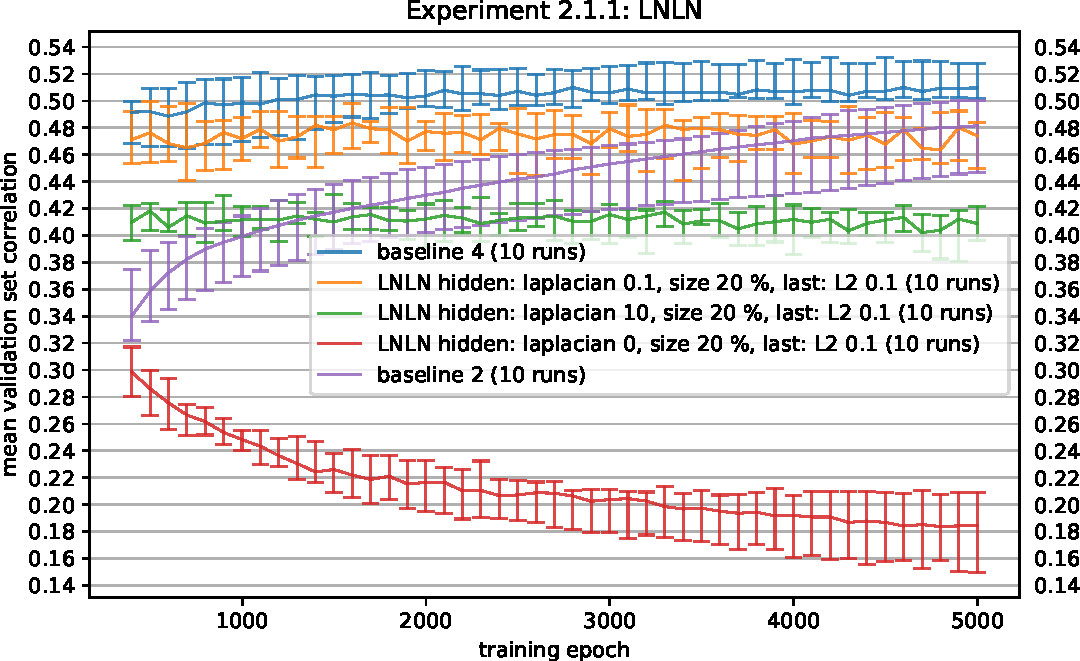
\includegraphics[width=1\textwidth]{../figures/05_2_1_1}
    \caption[Experiment 2.1.1]{Selected LNLN instances versus baseline 4 and 2.}
    \label{fig:5.2.1.1}
\end{figure}

The best instance achieved validation set correlation of (0.474, 0.484, 0.45) after 5 000 epochs (Fig. \ref{fig:5.2.1.1}). Despite being worse than \textit{baseline 4} (0.51, 0.527, 0.502), it was comparable to less fine tuned\footnote{While we tried to find optimal hyper-parameters, we did not have enough time to be confident saying this is the best or even close to the best result possible with this architecture. Significantly more time was spent on properly tuning the HSM architecture.} versions of our model, for example the \textit{baseline 2} (0.482, 0.5, 0.447). We believe this result is good evidence for the hypothesis that the biological constraints of HSM only serve as well fitting explicit regularizations that make the model more stable with respect to hyperparameters, but are not a necessity to achieve good results. A finding already supported by the state of the art results achieved by \cite{klindt} with a relatively more generic architecture.

A few more noteworthy observations. Moderately strong Laplacian regularization on the hidden layer was paramount. Without it, the model started overfitting very quickly and never recovered. The smaller hidden layer version, with the number of filters equivalent to 10 \% of the number of output neurons, had very similar performance characteristics to the larger version but was worse across the board. Too strong regularization, both on the hidden and the output layer, also caused lower performance.

\subsubsection{LN model}

\textit{Experiment 2.1.2} tested an architecture equivalent to a simple LN model. The first and only layer featured a spatial Laplacian regularization, with its strength being the only free hyperparameter of the architecture. 

\begin{figure}[H]
    \centering
    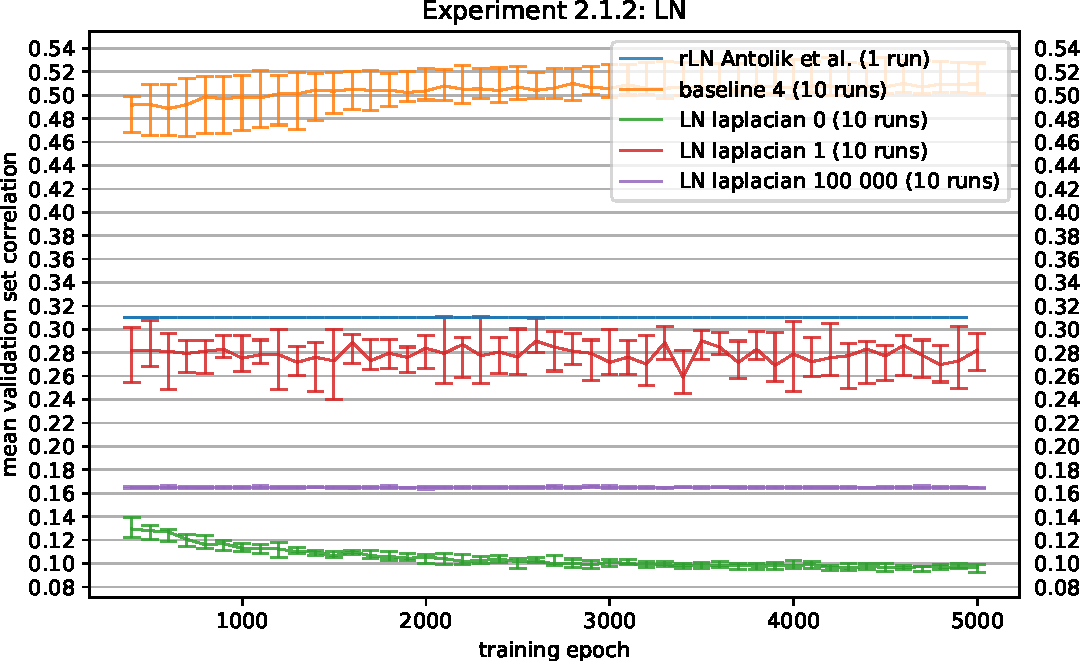
\includegraphics[width=1\textwidth]{../figures/05_2_1_2}
    \caption[Experiment 2.1.2]{Performance of LN-like model instances. Only a fully trained performance is available for the rLN model reported by \citeauthor{antolik}\protect\footnotemark.}
    \label{fig:5.2.1.2}
\end{figure}
\footnotetext{We only have fully trained data for the \citeauthor{antolik} rLN model. We thus show the final mean performance and its variance for all time points.}

As shown on figure \ref{fig:5.2.1.2}, the results (0.282, 0.296, 0.265) were substantially lower than those of our previously tested and more computationally complex models and on-par with the performance of an analytically optimized version of an LN model with Laplacian regularization reported by \cite{antolik} (0.31). The same as in the previous experiment, some regularization proved to be a necessity while too strong led to poor, albeit very consistent, performance.

\subsection{Convolutional and separable models}
\subsubsection{Convolutions instead of DoG}

In \textit{experiment 2.2.1}, we replaced the first DoG layer with a plain convolution featuring a Laplacian regularization. The rationale was twofold. First, we were inspired by the success of convolution based architectures as reported by \cite{klindt}, \cite{ecker}, \cite{Walke506956}, etc. Given this inspiration, we reintroduced a non-linearity after the convolution layer. Second, much like in \textit{experiment 2.1.1} with a fully connected layer, a convolution layer should be able to learn to represent anything the DoG layer can and as such might be viewed as just a more generic and less biologically constrained equivalent. We tested various sizes of the convolution (3 to 15 pixels), numbers of its filters (9 to 30), strengths of the Laplacian regularization, and additional L2 or max\footnote{For details, refer to section \ref{ch:3.1.1}.} regularization of the hidden fully connected layer. Convolution layer stride was set to half of the filter size.

\begin{figure}[H]
    \centering
    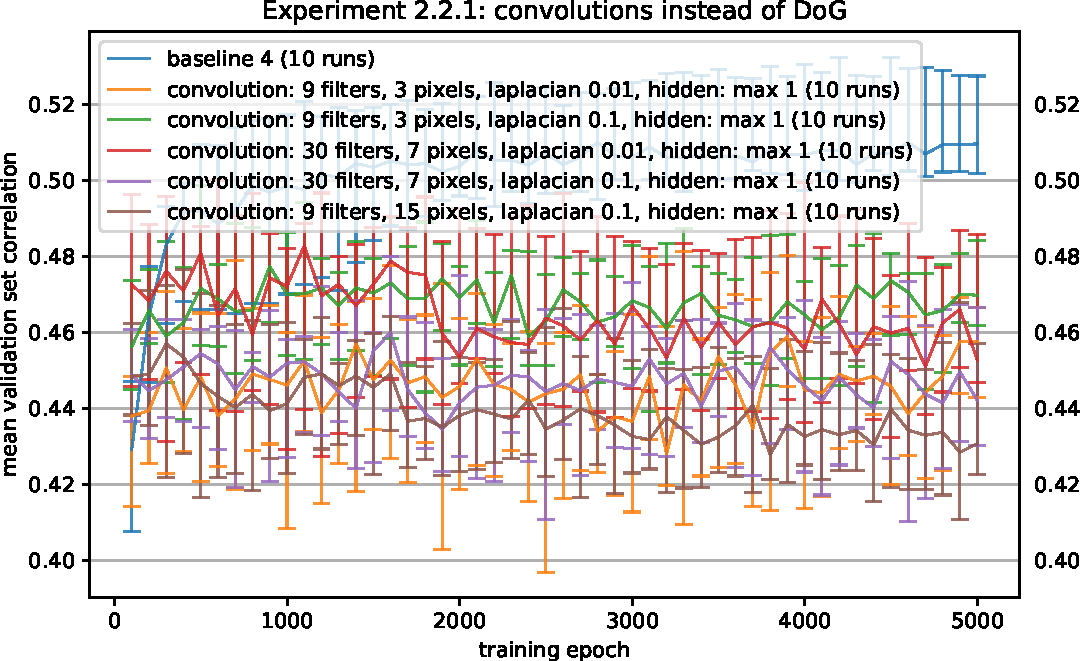
\includegraphics[width=1\textwidth]{../figures/05_2_2_1}
    \caption[Experiment 2.2.1]{Convolution layer with regularization instead of DoG layer.}
    \label{fig:5.2.2.1}
\end{figure}

The results (Fig. \ref{fig:5.2.2.1}) were similar to those of the LNLN model experiment, with the best model achieving validation set correlation of (0.47, 0.484, 0.462) by the end of training. Both instances with 9 filters and 30 fared very similarly. For filter size, both small, 3 pixels wide, and moderate, 7 pixels wide, convolutions reached decent performance, with large filters of 15 pixels being significantly worse (0.431, 0.457, 0.423). Strong max regularization on the hidden layer proved to be a necessity for high performance. In contrast, L2 overwhelmed the training even on the lowest tested strength. 

Some observations were hard to interpret, such as the interaction of Laplacian regularization on the convolution layer and the layer’s filter size. While a stronger variant worked better on a smaller convolution layer with 9 3-pixels wide filters, it worked - by roughly the same amount - worse on a larger 7-pixels wide 30 filters instance. A result that is the exact opposite of what we would expect, given the intuition that larger and more numerous filters have more opportunity to overfit and so might require stronger regularization. We hypothesize that, as regularizations in NDN3 are not normalized to layer size, the larger the layer, the higher the chance a regularization on it will overwhelm the loss function and thus negatively impact training. On the other hand, for the largest convolution filters - 15 pixels wide, stronger laplacian regularization proved to be beneficial again. A more thorough investigation of this issue would be needed to draw conclusions. At least some Laplacian regularization on the convolution filters was a necessity, however. Without it, the best model reached (0.242, 0.281, 0.209) with clear signs of overfitting.

\subsubsection{Convolutions and separable}

Experiment 2.2.2 built on the architecture of 2.2.1, only replacing the hidden fully connected layer with a separable layer as it was introduced by \cite{klindt}\footnote{For details, refer to section \ref{ch:2.2}.}$^{,\thinspace}$\footnote{There are still large differences between this experiment’s architecture and \cite{klindt} model. Namely in the number of sequential convolution filters (1 vs 3), absence of batch normalisation, different regularization, and two-layer readout (hidden and output) instead of just a single separable layer.}. This test was motivated by the improvements reported by \citeauthor{klindt} where the separable readout layer increased validation set correlation on region 1 from 0.47 to 0.55 over a fully connected variant. Due to unavailability of max regularization for the separable layer, this test assessed L1 and L2 regularizations for the hidden layer.

These changes led to better results (Fig. \ref{fig:5.2.2.2}), with the best instance reaching peak of (0.494, 0.51, 0.462) and end of training performance of (0.474, 0.499, 0.461). In contrast to the fully connected variant from 2.2.1, small convolution filters had worse performance than larger ones - with 3-pixels wide being substantially less effective. This was a surprise as we only changed the readout mechanism of the hidden layer and as such did not expect the interactions of the first layer to be different. The number of filters had, as in the previous experiment, little effect.

\begin{figure}[H]
    \centering
    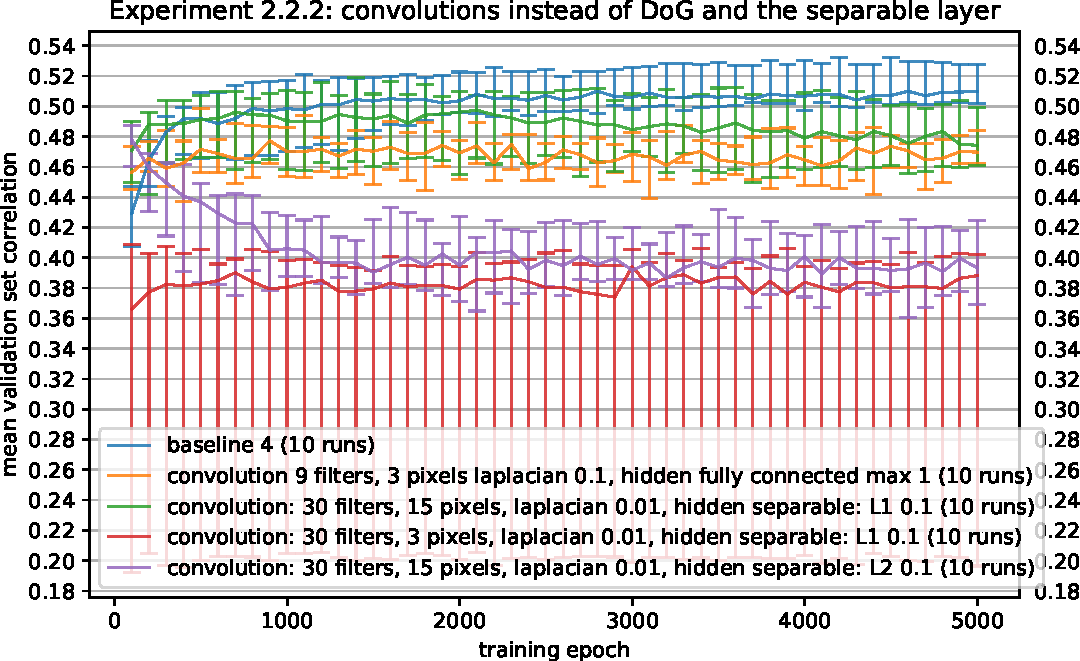
\includegraphics[width=1\textwidth]{../figures/05_2_2_2}
    \caption[Experiment 2.2.2]{Convolution and separable hidden layer.}
    \label{fig:5.2.2.2}
\end{figure}

We also observed another instance (see experiment 2.2.1) of non-additivity of regularization benefits. Moderate L1 on hidden and Laplacian on the convolution worked best, followed by either of them stronger and the other weak, with both of them strong as the least performant variant. L2 regularization on the hidden layer led to significantly worse results across the board.

\subsubsection{Convolutional DoG}

With \textit{experiment 2.2.3}, we tested two further variants of this architecture. Both featured a convolutional variant of the DoG layer as the first filter layer and had either a fully connected or separable layer as the hidden layer. The tested variants were the same as in \textit{2.2.1} and \textit{2.2.2} with the obvious lack of Laplacian regularization on the filter layer - as the convolutional variant of DoG implicitly features a hard regularization of its filters.

The rationale behind a convolutional variant of the DoG layer was as follows. Optimizing the locations of centers of difference-of-Gaussians within the DoG layer through gradient descent is not optimal. If the random initialization puts the center completely outside of where it should be, it is unlikely\footnote{Based on our very limited testing of learning properties of the DoG layer. To draw any conclusions, we suggest further research on the interaction between gradient descent based optimizers and the DoG layer.} the gradient for respective location parameters overweights the rest and changes the position substantially\footnote{Fortunately, given the number of filters and size of our input images, this never proved to be an issue on our dataset.}. At the same time, the locational invariance of V1 neurons leveraged through convolution layers by Klindt et al. and Ecker et al. should work with explicitly parameterized difference-of-Gaussians filters just as well as with generic filters.

\begin{figure}[H]
    \centering
    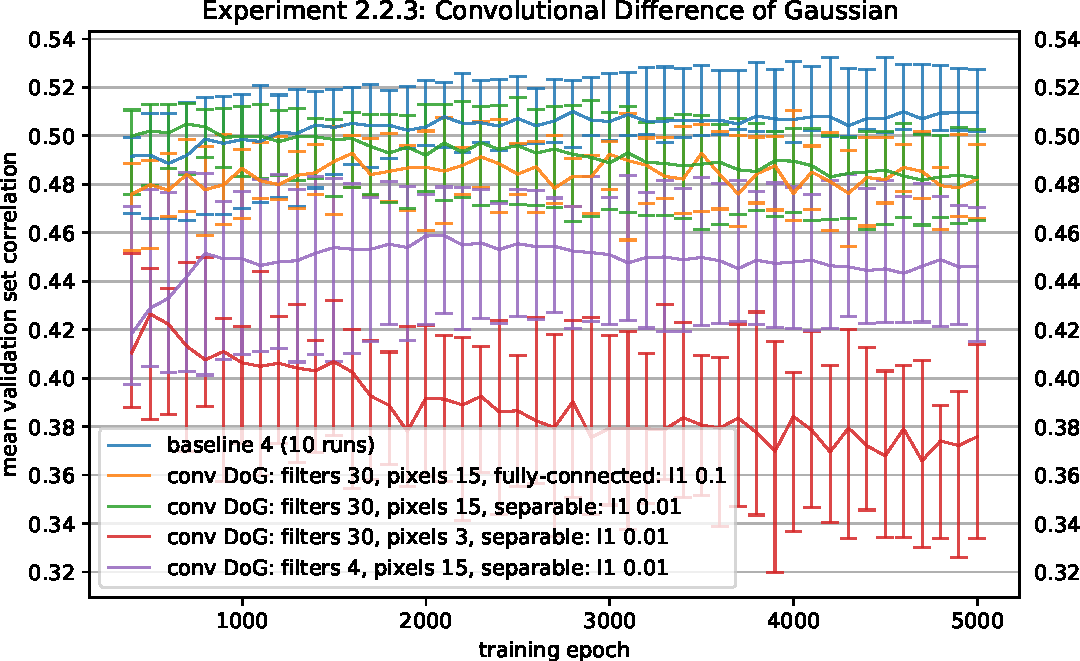
\includegraphics[width=1\textwidth]{../figures/05_2_2_3}
    \caption[Experiment 2.2.3]{Convolutional variants of the DoG layer.}
    \label{fig:5.2.2.3}
\end{figure}

Both versions, with a fully connected as well as a separable hidden layer, achieved a similar level of performance (Fig. \ref{fig:5.2.2.3}), (0.482, 0.496, 0.466) and (0.483, 0.502, 0.465) respectively, that was comparable to a number of recent models such as the convolution variants \textit{(2.2.2)}. The best instance of the separable version reached a peak of (0.498, 0.51, 0.484) and showed signs of overfitting. For both versions, small 3pixels wide DoG filters did not perform well\footnote{Similar to the separable version of convolutional variant \textit{(2.2.2)} but unlike the fully connected version of convolution variant \textit{(2.2.1)}. A plausible explanation is that 3x3 pixels is not enough to fully realize a difference-of-Gaussians filter.}, with the widest 15pixels getting the best results. The number of filters had, as in the previous experiments, relatively low influence with 30 filters achieving initially higher results and then falling, likely due to overfitting.

Notably, the instances with only 4 filters fared substantially worse than their 9 filter counterparts. This was a relatively surprising result. Since 9 filters were enough for a non-convolutional DoG variant, where each filter contains a single difference-of-Gaussians at a specific location, we assumed that the convolutional variant that applies each difference-of-Gaussians filter at multiple locations might work with a smaller number of filters. In essence, we assumed that the computation requires a very few types of filters applied at multiple locations instead of a very specific filter for each of relatively few locations. This result, instead, suggests nearby neurons within V1 indeed pool from a rather limited number of LGN inputs that are backed by very specific locations and receptive field topologies within the visual field. We suggest further investigation of the trained weights of this architecture and comparison to the fully connected versions as well as the original HSM version with plain DoG layer.

For the fully connected versions, both L1 and max regularizations worked similarly. The separable version performed best with a light L1 regularization, with L2 overwhelming the training.

\subsubsection{Convolutional variants without non-linearity}

\textit{Experiment 2.2.4} investigated the effect of the nonlinearity after the convolutional DoG filter layer on both variants, with a separable as well as fully connected hidden layer. In contrast to convolutional models by others such as those reported by \cite{klindt} or \cite{ecker}, where multiple nonlinearities worked well, for our architecture the variants without a nonlinearity achieved slightly higher results.

\begin{figure}[H]
    \centering
    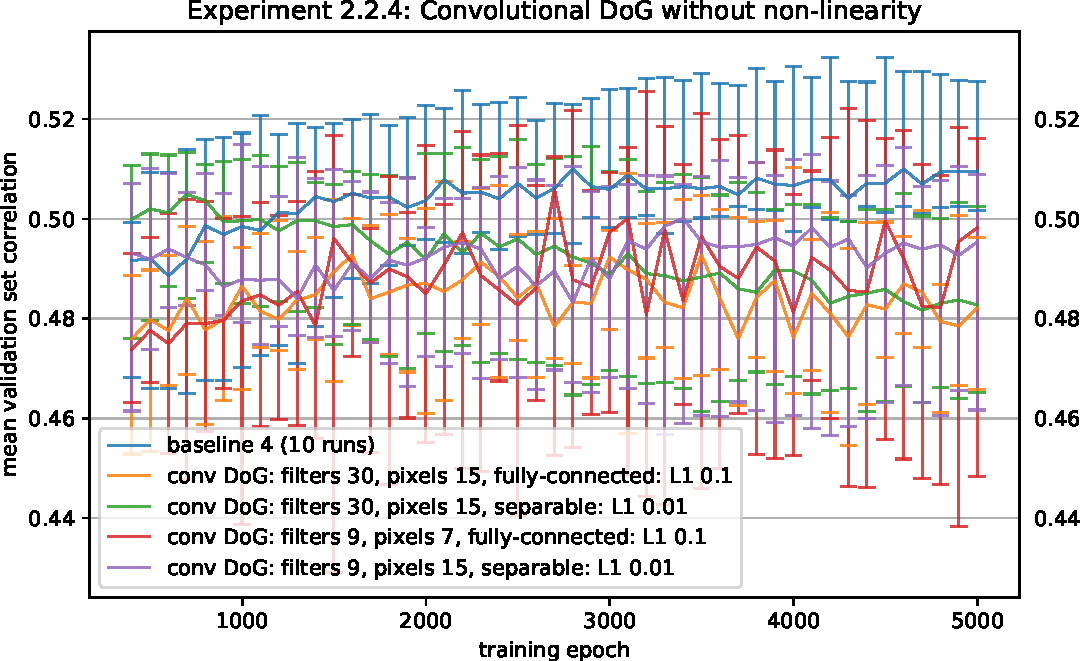
\includegraphics[width=1\textwidth]{../figures/05_2_2_4}
    \caption[Experiment 2.2.4]{Filter layer non-linearity and the convolutional DoG variant.}
    \label{fig:5.2.2.4}
\end{figure}

While still lower than our baseline model, the linear version of a fully connected hidden layer variant achieved (0.498, 0.516, 0.448) versus (0.482, 0.496, 0.466) of the nonlinear version (Fig. \ref{fig:5.2.2.4}). And the separable version reached (0.495, 0.509, 0.462) versus (0.483, 0.502, 0.465) of its nonlinear counterpart. Surprisingly, a variant with 7 pixels wide convolutions performed best for the linear activation function version of a separable variant, while 15 pixels filters worked best for all other versions. As in previous experiments, we invite further research into the exact form of the trained filters. Informed by these and \textit{1.3.4} results, we also suggest investigating the exact effects of the number of nonlinearities in the model across various architectures.

\subsubsection{Reimplementing what/where model}

Entirely as an exercise, with \textit{experiment 2.2.5} we tried to reimplement the what/\-where model architecture as introduced by \cite{klindt} Due to it not being the focus of our work, we limited ourselves to only information published in the paper without consulting either of the available implementations\footnote{\href{https://github.com/david-klindt/NIPS2017}{https://github.com/david-klindt/NIPS2017}, \\ \href{https://github.com/aecker/cnn-sys-ident/tree/master/analysis/iclr2019}{https://github.com/aecker/cnn-sys-ident/tree/master/analysis/iclr2019}.}. Given that, we had to grid-search some hyperparameters such as regularization strengths or convolution strides and also chose to use our training regime. 

Further, we replicated the architecture using only techniques already available in NDN3, which forced us to deviate from the original in a number of ways. Instead of the in-NDN3-unavailable group-sparsity regularization on the 3 convolutional layers cascade, we tested max and L2 regularizations. For the same reason, we had to leave out batch normalisation which is originally part of each convolutional layer of the model. Generally, our version was relatively different in terms of things that influence training but was equivalent inference architecture wise.

The best instance reached peak validation set correlation of (0.48, 0.497, 0.461) and (0.479, 0.494, 0.455) at the end of training (Fig. \ref{fig:5.2.2.5}). A result on par with our shallower convolution variant of the HSM model (experiment 2.2.2) but still below both our baseline 4 model and especially the published result of 0.55 of the original \citeauthor{klindt} version. As this was a sideline exercise, we did not dedicate further resources to properly reimplement the model. However, we still believe it can serve as evidence that hyperparameters and only training influencing parts of the model can have more substantial impact than larger architectural differences.

In addition to hyperparameters that were in accordance with the paper, we also tested a few other variants. Interestingly, with this architecture L1 regularization worked better than L2 on the output layer. A complete opposite to what we observed on our HSM based models. We also observed that 2-pixel strides on the convolutional layers worked consistently better than half-the-filter-size strides. A result suggesting fine-tuned positioning of first layer filters is important.

\begin{figure}[H]
    \centering
    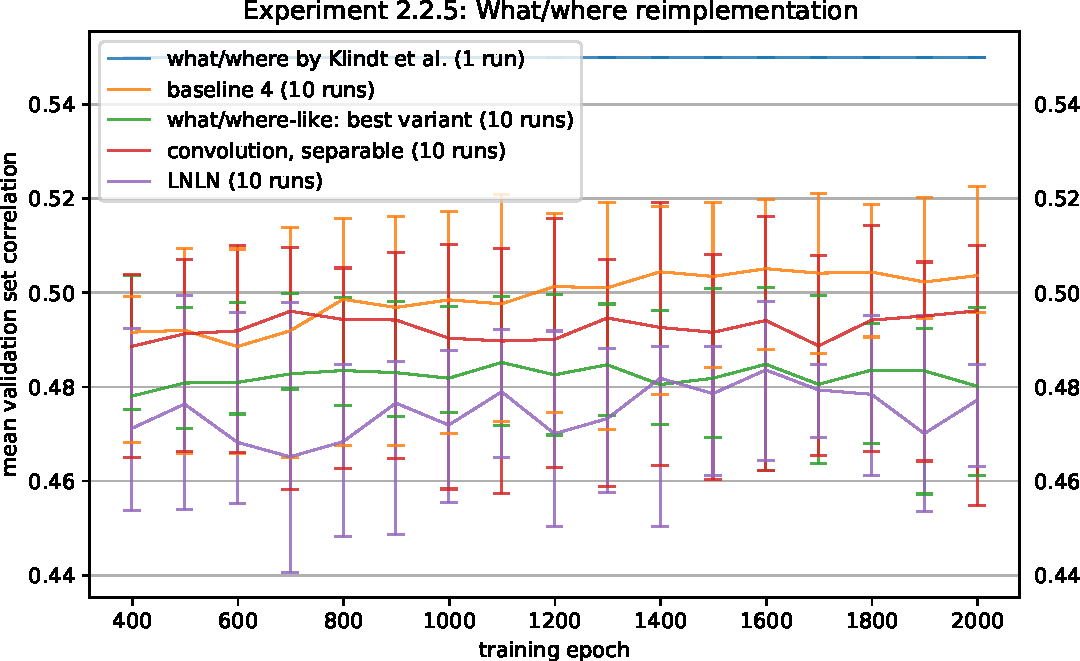
\includegraphics[width=1\textwidth]{../figures/05_2_2_5}
    \caption[Experiment 2.2.5]{Comparing the best reimplemented what/where instance to various other model architectures.}
    \label{fig:5.2.2.5}
\end{figure}

\subsection{Discussion}

The theme of this section’s experiments could be summarized as testing various computationally equivalent architectures. The observed difference between different types of either the first or the second layer was relatively small (Fig. \ref{fig:5.3.2.1_1}). At least when we assumed the best performing instances and in comparison to the variance within one architecture across different hyperparameter combinations. All three versions of the first layer fared very similarly in terms of achieved correlation on the validation set. The plain DoG variant, our baseline, remained the highest performing. But the difference was so small it could also be explained by not as involved finetuning of hyperparameters for the other variants as was done for the baseline model\footnote{Across both the first section experiments and also the original \cite{antolik}}. For this reason, we decided not to test small variations of either of the DoG layers versions, for example with only one Gaussian, a not-concentric version, etc. 

This result was, in a way, expected. All tested alterations are theoretically computationally equivalent. Or rather, all variants can learn to compute whatever the plain version of the DoG layer can. Its convolutional variant is just a positional relaxation of it, the normal convolutional layer sheds the hard regularization constraint on the filter weights, and the LNLN variant just goes one additional step further removing the factoring into two layers. A more surprising observation was that the convergence speed and its progression were also similar. After all, the main difference was that certain variations imposed priors in the form of hard/soft regularization on the layers, which we assumed would heavily impact convergence. While a more thorough investigation would be needed, the similar but not better performance of alternatives serves as evidence that the plain difference-of-Gaussians restriction on the first layer filter might be correct but also is not necessary.

\begin{figure}[H]
    \centering
    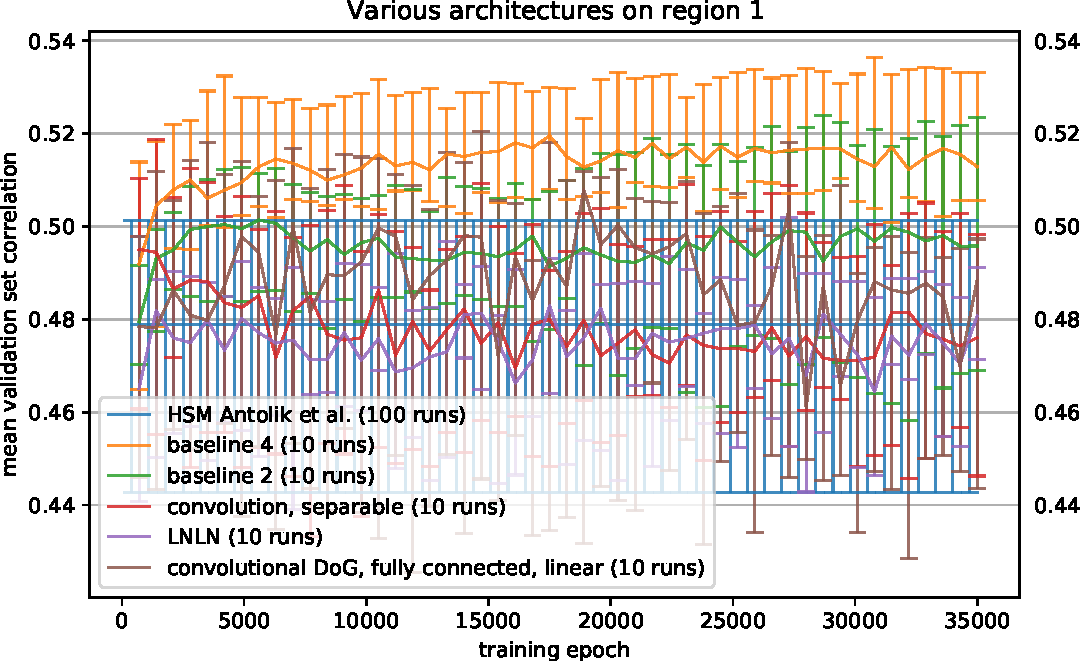
\includegraphics[width=1\textwidth]{../figures/05_3_2_1_1}
    \caption[Various architectures on region 1]{Various architectures fully trained on region 1.}
    \label{fig:5.3.2.1_1}
\end{figure}

The small observed difference between the variation with a fully connected hidden layer and a variant with a separable layer was also relatively surprising Based on the improvements reported by \cite{klindt} on their architecture, where using it increased the best-achieved performance from 0.47 to 0.55 on region 1, we were surprised by the, in comparison, smaller improvements on our plain convolution variant and almost negligible differences on the convolutional DoG version. It is, however, important to note that there are relatively big architectural differences between those two architectures, such as 1 filter versus 3 filters cascade and an additional fully connected output layer after the readout layer.

Both of the aforementioned results could be further researched. It would be especially interesting to compare the trained weights of the first layer filters and second layer masks between individual variants and figure out if they only lead to comparable levels of performance or if they are, in fact, equivalent computation-wise. Going even deeper, a comprehensive comparison between the hard regularizations - such as the of DoG layer - and various soft regularizations like a Laplacian regularization on a convolutional layer, could also lead to interesting discoveries. 

Similarly, the question of why exactly does adding a non-linearity after the first layer cause diminished performance on our HSM-based architecture but seems to work for deeper models, could also be explored further in at least two ways. First, as a general ML research on the ability of a smaller network to deal with a redundant non-linearity. And second, as a more neuroscience inspired investigation into the question of whether the computation being modeled might actually be as simple as requiring only two non-linearities, with the goal of informing our understanding of visual computation processes.


In agreement with our observations regarding high-level architecture versus hyperparameters tuning and training time details, we also did not manage to achieve published results with our relatively close reimplementation of the what/where model by Klindt et al. This was mostly due to it being just an afterthought exercise without enough resources allocated to it, but it can, in our opinion, still serve as evidence of the importance of careful tuning. 

We suggest further inquiry in the comparison of multilayer filters, such as those of Klindt et al. architecture, and single-layer filters of our HSM-based approach. Especially in the face of our aforementioned findings that additional nonlinearity leads to diminished performance in our HSM-based models while the what/where model features a cascade of 3 convolutions, each followed by a non-linearity. 

\section{All regions experiments}

In this section, we make use of all three regions of the dataset (see section \ref{ch:4.1.1}). First, we pool the regions together and test one shared model trained on all data. Second, we assess how various architectures explored in previous sections work on regions 2 and 3 and investigate how well our observations made on region 1 generalize.

\subsection{Combined dataset}\label{ch:5.3.1}
\subsubsection{Region pooled dataset}

\textit{Experiment 3.1.1} explored pooling multiple regions together to train a single model on higher quantity of data. The rationale behind this was the same as why record and then subsequently fit multiple neurons from a single V1 region at the same time, instead of fitting them one by one separately\footnote{Notably, the LN/rLN model is effectively fitted per neuron.}. While the similarity in both inputs and computational properties is lower between V1 neurons from different regions than within a region, it is still there and - to a lesser degree - is even present across neurons from multiple individuals, such as between regions 1,2 and region 3. Training one model across data from multiple regions can then help ground the common computation, thus mitigating the effect of random noise that is present in the data, and improve the accuracy of the trained model. All models trained in this experiment were based on baseline 3. 

To assess the benefits of this approach, we first needed a baseline model that does not involve any data sharing between regions. We created an ensemble of three separate models, each trained on and responsible for predicting one of the three regions. To measure its performance, we used the average of validation set correlations across the three regions weighted by the number of output neurons in each. Thus, getting an unbiased per neuron average validation set correlation across all available data.

The shared model was trained on all three regions using the data filters capability of NDN3 (see section \ref{ch:3.1.1}). As such it effectively shared the first two layers, DoG filter and fully connected hidden, between all neurons from all three regions and had per output neuron\footnote{Alternative interpretation is that we are effectively using transfer learning across the tree regions. Pre-training the first two layers of the model on all three regions together and then adding and fine tuning the last layer for each region individually.} - and thus also per region - output. Since more data was being fit, the assumption was that the model might need bigger capacity and potentially stronger regularization. To test this, we trained variants with 9 to 25 DoG filters, hidden layer sizes of 20 \% and 30 \% of the number of output neurons\footnote{Across all three regions.}, and various strengths of L2 regularization on both the hidden and the output layers. 

The best instance of the model trained on all three regions pooled together achieved worse performance than its separate-models-ensemble counterpart (Fig. \ref{fig:5.3.1.1_1}), with end of training validation set correlation of (0.439, 0.459, 0.426) versus (0.474, 0.486, 0.46). 

\begin{figure}[H]
    \centering
    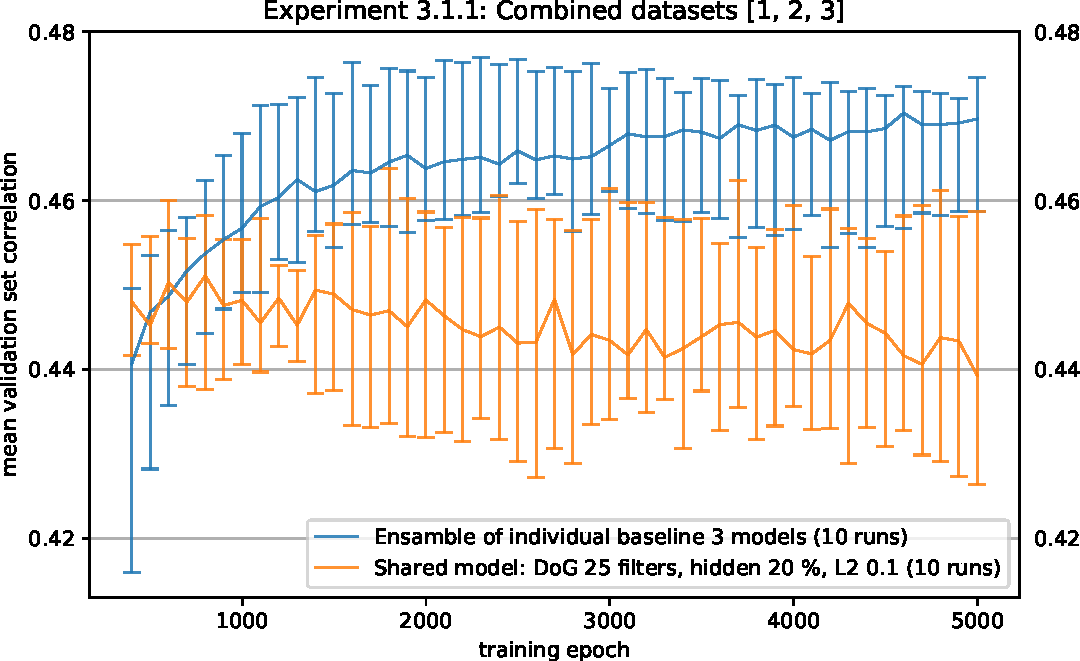
\includegraphics[width=1\textwidth]{../figures/05_3_1_1_1}
    \caption[Experiment 3.1.1]{Models trained on regions 1,2,3 pooled together\protect\footnotemark.}
    \label{fig:5.3.1.1_1}
\end{figure}
\footnotetext{Shared model represents a single model trained on data pooled together, the ensemble is just a weighted average of three separate models.}

In addition to using all three regions, we also run the same experiment with only the first two regions pooled together, thus limiting ourselves to data recorded from the same animal\footnote{Regions 1 and 2 were recorded using one animal, region 3 with another.}. In contrast the three-regions-variant, the model trained on only regions 1 and 2 pooled together reached correlation of (0.484, 0.495, 0.471), beating (0.475, 0.483, 0.475) of its 2-models-ensemble baseline (Fig. \ref{fig:5.3.1.1_2}).

\begin{figure}[H]
    \centering
    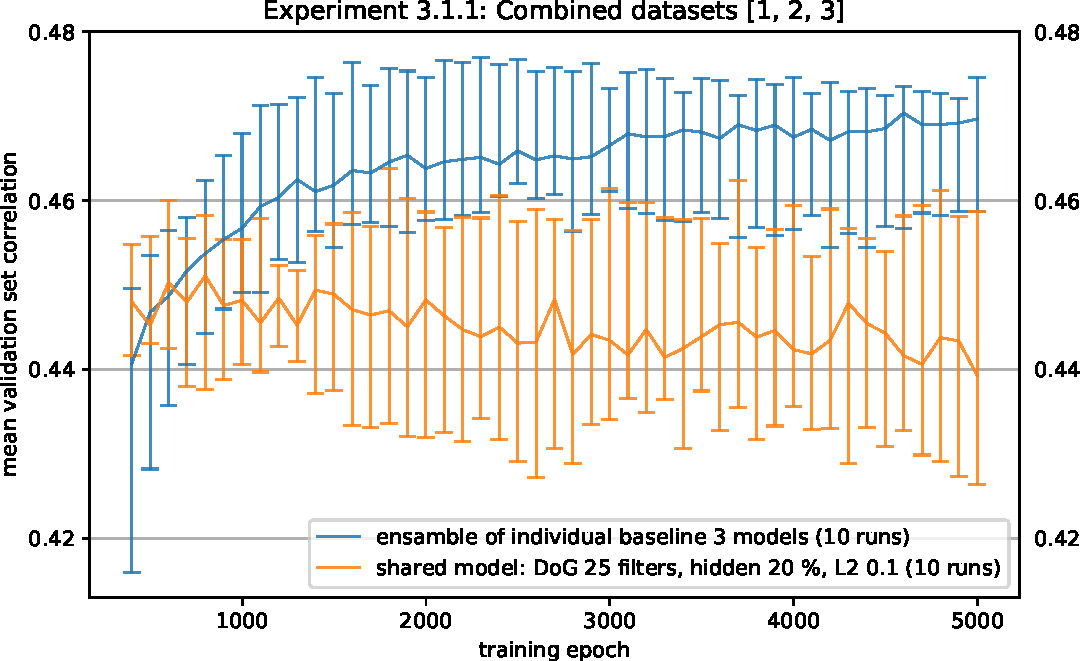
\includegraphics[width=1\textwidth]{../figures/05_3_1_1_2}
    \caption[Experiment 3.1.1 2]{Models trained on regions 1,2 pooled together\protect\footnotemark.}
    \label{fig:5.3.1.1_2}
\end{figure}
\footnotetext{Shared model represents a single model trained on data pooled together, the ensemble is just a weighted average of two separate models.}

The simplest explanation of this phenomenon would be that the model, when shared across all three regions, did not have enough capacity to handle all the data. Since the hidden layer was proportional to the number of output neurons and we even tested a larger variant - with worse results, it was unlikely\footnote{It is possible that we might also be experiencing critical regime of deep double descent phenomena (\cite{2019arXiv191202292N}).} to be the cause. Similarly, we did not observe differences between variants with 15 and 25 DoG filters that would suggest even more filters were needed. Performance of variants with various levels of L2 regularization on both fully connected layers also did not provide evidence for insufficient regularization. 

With insufficient model capacity and regularization out of the way, several data focused hypotheses explaining these results remained. Notably, the third region was recorded using a different animal and so it is possible the similar computation properties assumption, as declared above, only holds within one animal. Following similar logic, it is possible that the noise distribution across the three regions substantially varies as well. A more thorough exploration would be needed to draw any conclusions, however. Specifically, we suggest further inquiry in the individual region performance of our pooled regions models and a more in depth investigation of the differences between the tree regions data.

A few additional observations. Models trained on pooled regions required more DoG layer filters than the 9 presented in the per-region models, and, with that, benefited from L2 regularization on both the output as well as the hidden fully connected layers. Stronger L2 regularization coupled with only 9 filters led to very poor performance. 

\subsection{Testing on other regions}\label{ch:5.3.2}
\subsubsection{Various architectures across regions}

We finish this chapter with \textit{experiment 3.2.1} that assessed various architectures from previous sections on each of the three regions. We trained 5 models: \textit{baseline 2 (1.2.1)}, \textit{baseline 4 (1.3.3)}, the best \textit{LNLN instance (2.1.1)}, the best \textit{convolution instance (2.2.2)}, and the best \textit{convolutional DoG instance (2.2.4)}. Each was trained fully for 35 000 epochs with 10 runs. The motivation was to compare how various architectures fare and if their (relative) performance is stable across different regions

The baseline models with plain DoG layer outperformed all other variants across all three regions (Figs: \ref{fig:5.3.2.1_1}, \ref{fig:5.3.2.1_2}, \ref{fig:5.3.2.1_3}, table \ref{tab:5.3.2.1}). However, the improvements of \textit{baseline 4} with respect to both the original reported Antolik et al. implementation and our \textit{baseline 2} model did not translate to regions 2 and 3. Especially on region 2, the difference between \textit{baseline 4} (0.414, 0.434, 0.407) and numbers reported by Antolik et al. (0.412, 0.435, 0.382) was negligible for 90th and 50th percentile, with improvements only in the 10th percentile run. On region 3, the baseline models fared better but \textit{baseline 2} model actually outperformed \textit{baseline 4}.

\setlength{\abovecaptionskip}{10pt plus 0pt minus 0pt} % Chosen fairly arbitrarily
\begin{table}[H]
    \renewcommand{\arraystretch}{1.0}
    \centering
    \begin{tabular}{l|l|l|l}
        \toprule
        \textbf{Model} & \textbf{Region 1} & \textbf{Region 2} & \textbf{Region 3} \\ \midrule
        \citeauthor{antolik} & 0.479, 0.501, 0.442 & 0.412, 0.435, 0.382 & 0.437, 0.449, 0.419 \\ 
        Baseline 4 & 0.513, 0.533, 0.506 & 0.414, 0.434, 0.407 & 0.449, 0.455, 0.439 \\ 
        Baseline 2 & 0.496, 0.523, 0.469 & 0.415, 0.429, 0.398 & 0.454, 0.460, 0.449 \\ 
        Convolution & 0.476, 0.498, 0.446 & 0.358, 0.391, 0.306 & 0.416, 0.445, 0.403 \\ 
        LNLN & 0.481, 0.491, 0.471 & 0.340, 0.362, 0.327 & 0.404, 0.417, 0.396 \\ 
        Conv. DoG & 0.486, 0.499, 0.450 & 0.318, 0.363, 0.288 & 0.396, 0.432, 0.384 \\ \bottomrule
    \end{tabular}
    \caption[Performance of various models across regions]{Validation set correlations (50th, 90th, 10th percentiles) of various architectures across three regions.}
    \label{tab:5.3.2.1}
    \renewcommand{\arraystretch}{1.0}
\end{table}
\setlength{\abovecaptionskip}{0pt plus 0pt minus 0pt} % Chosen fairly arbitrarily

While on region 1 all models, apart from \textit{baseline 4}, fared relatively similarly - with 50th percentile runs in the range of 0.476-0.496, on regions 2 and 3 there were two separate groups. With higher performance, there were the variants with plain DoG layer (baselines 2, 4 and the original \cite{antolik}\footnote{Further referred to as the HSM architecture}) and with a significant gap and lower performance all the other architectures (convolution, convolutional DoG, and LNLN). The relative performance in the lower group was not stable across regions either, with convolutional DoG model performing worst on region 2 but very comparably to others on regions 3 and 1. 

\begin{figure}[H]
    \centering
    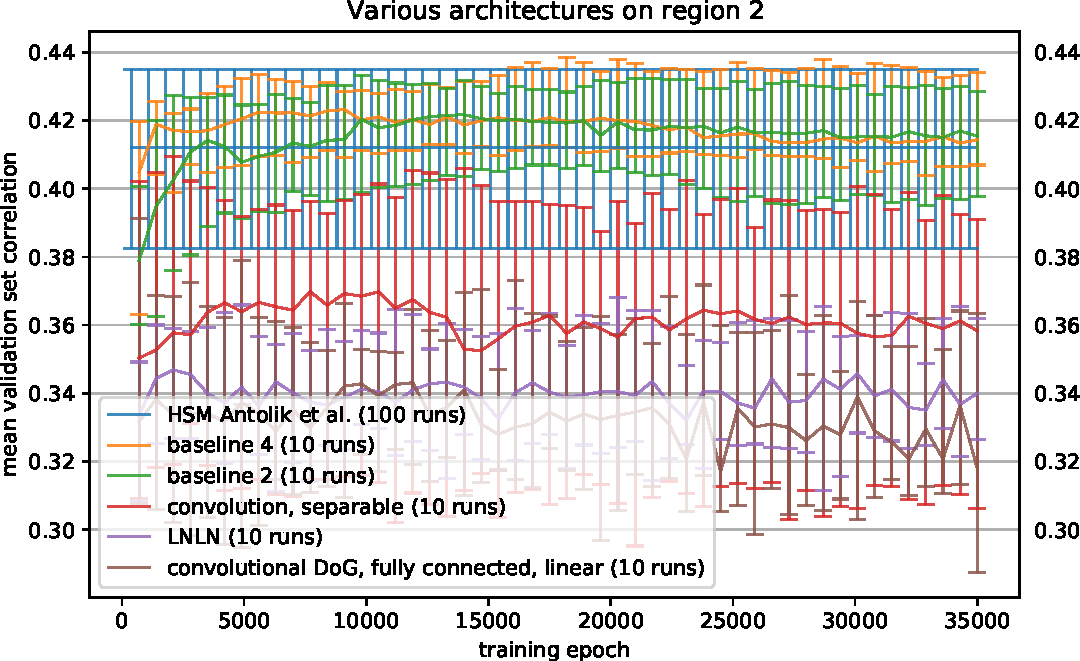
\includegraphics[width=1\textwidth]{../figures/05_3_2_1_2}
    \caption[Various architectures on region 2]{Various architectures trained on region 2.}
    \label{fig:5.3.2.1_2}
\end{figure}

\begin{figure}[H]
    \centering
    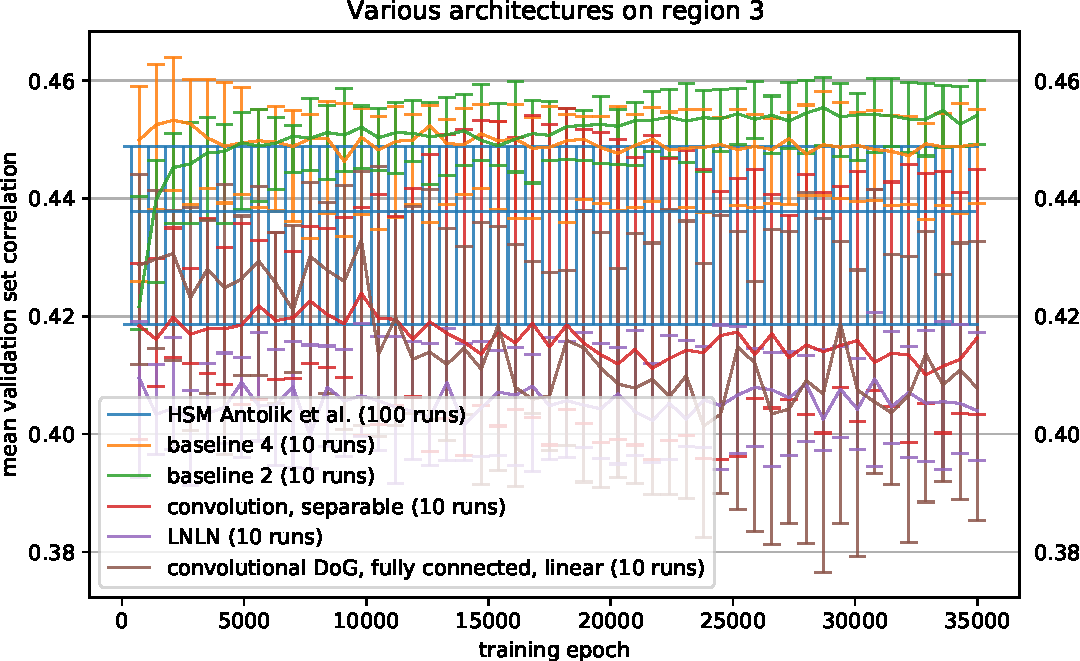
\includegraphics[width=1\textwidth]{../figures/05_3_2_1_3}
    \caption[Various architectures on region 3]{Various architectures trained on region 3.}
    \label{fig:5.3.2.1_3}
\end{figure}

The convolutional variants (convolution and convolutional DoG) exhibited two noteworthy behaviours. First, they suffered overfitting on region 3. This was puzzling since, region 3 is of the same size as region 1, with region 2 being relatively smaller and thus - as we would expect - more susceptible to overfitting. Second, they were significantly less consistent in stability with respect to random initialization across the three regions. This showed especially on region 2 but was relatively clear even on region 3. Surprisingly, the LNLN architecture seemed relatively well behaved in this regard, with its 10-90th percentile run range consistent and comparable to the plain DoG layer variants across all three regions.

Given the big difference between plain DoG variants and both of the convolutional architectures together with the LNLN model, we suspect the main benefit of the plain HSM architecture over convolutional variants, when it comes to robustness across multiple similar datasets without further fine-tuning, is in the very limited number of outputs from the first filter layer. That said, we were surprised the separable hidden layer present in the convolution model did not achieve a similar effect. On similar note, we expected the hard regularization of the convolutional DoG architecture or the location invariant properties of the plain convolution model to also positively influence robustness in comparison to the very generic LNLN model. 

A more thorough investigation would be needed to draw any conclusions. We especially recommend looking into the trained weights of each architecture and comparing them across the three regions. Repeating some of the grid-search experiments to fine-tune hyperparameters of the convolutional architectures on regions 2 and 3 might also bring relevant data. For now, however, we believe these results can still serve as evidence for the robustness of the original HSM architecture with its plain non-convolutional DoG layer.

\subsection{Discussion}

In this section, we made two important findings. First, pooling separately record\-ed regions together to train a single shared model did not provide expected benefits. On the contrary, for the version with all three regions pooled together, it led to worse performance than a simple ensemble of three separate models. To make things more convoluted, this method achieved slightly better results than the ensemble baseline when only the first two regions were pooled. 
This suggests the intriguing hypothesis that the pooling of the data across regions might work within an animal but not across animals, as regions 1 and 2 were recorded in the same animal, while region 3 in a different one. 

Our conclusion is that in our hands, pooling of data across multiple recordings does not impart advantage over fitting models individually. It is, however, important to emphasize that this conclusion is strictly specific to the data available in this thesis and to our current level of understanding of both the dataset and the modeled computation.

Second, we found heterogeneity of outcomes when testing various architectures, fine-tuned on region 1 in the previous sections, on regions 2 and 3. Our improvements of the HSM architecture with baseline models proved not to be universal, with, for example, baseline 2 achieving higher than \textit{baseline 4} on region 3. We also found that architectures with a plain DoG layer were generally more robust when it comes to transferring them to similar, but not equal, datasets without further hyperparameters fine-tuning. In contrast to this finding, we did not observe similar benefit to either the convolutional DoG variant or plain convolution variant with a separable readout layer over a simple LNLN architecture.

\setlength{\abovecaptionskip}{10pt plus 0pt minus 0pt} % Chosen fairly arbitrarily